\documentclass[10pt,a4paper]{article}
\usepackage{comment}
\usepackage{geometry}
\usepackage{graphicx}
\usepackage{amsthm,amsfonts,mathrsfs}
\usepackage{enumerate}
\usepackage{amsmath,accents}
\usepackage{amsfonts}
\usepackage{amssymb}
\usepackage{relsize}
\usepackage{latexsym}
\usepackage{subfigure}
\usepackage{hyperref}
\usepackage{nomencl}
\usepackage[dvipsnames]{xcolor}
\usepackage[normalem]{ulem}
\usepackage{bold-extra}
\usepackage{tikz}
\usetikzlibrary{shapes,arrows}
\tikzstyle{decision} = [diamond, draw,
    text width=4.5em, text badly centered, node distance=3cm, inner sep=0pt]
\tikzstyle{block} = [rectangle, draw, fill=blue!20,
    text width=5em, text centered, rounded corners, minimum height=4em]
\tikzstyle{line} = [draw, -latex']
\tikzstyle{cloud} = [draw, ellipse,fill=red!20, node distance=3cm,
    minimum height=2em]
\setlength{\parindent}{0pt}

\newcommand{\nomunit}[1]{\renewcommand{\nomentryend}{\hspace*{\fill}#1}}

\newcommand{\partder}[2]{\ensuremath{\frac{\partial #1}{\partial #2}}}
\newcommand{\secpartder}[2]{\ensuremath{\frac{\partial^2 #1}{\partial #2^2}}}
\newcommand{\nthpartder}[3]{\ensuremath{\frac{\partial^{#1} #2}{\partial #3^{#1}}}}
\newcommand{\fullder}[2]{\ensuremath{\frac{\mbox{d} #1}{\mbox{d} #2}}}
\newcommand{\secfullder}[2]{\ensuremath{\frac{\mbox{d}^2 #1}{\mbox{d} #2^2}}}
\newcommand{\nfullder}[3]{\ensuremath{\frac{\mbox{d}^{#1} #2}{\mbox{d} #3^{#1}}}}
\newcommand{\mixedder}[3]{\ensuremath{\frac{\partial^{2} #1}{\partial #2 \partial #3}}}
\newcommand{\df}[1]{\, \ensuremath{\mbox{d}#1}}
\newcommand{\grad}{\, \mbox{grad} \,}
\newcommand{\dive}{\, \mbox{div} \,}
\newcommand{\real}[1]{\text{Re} \left\{ #1 \right\}}
\newcommand{\imag}[1]{\text{Im}\left\{ #1 \right\}}
\newcommand{\commentstm}[1]{\textcolor{blue}{\textbf{STM:\ #1}}}
\newcommand{\commentstmtwo}[1]{\textcolor{purple}{\textbf{STM:\ #1}}}
\newcommand{\newstm}[1]{\textcolor{red}{\textbf{#1}}}
\newcommand{\newstmtwo}[1]{\textcolor{orange}{\textbf{#1}}}
\newcommand{\oldstm}[1]{\sout{#1}}
\newcommand{\oldstmtwo}[1]{\xout{#1}}

\newcommand{\brok}{\textcolor{ForestGreen}{\textit{\textbf{OK for Bernhard}}}}
\newcommand{\apok}{\textcolor{ForestGreen}{\textit{\textbf{OK for Andr\'{e}}}}}
\newcommand{\brnok}{\textcolor{red}{\textit{\textbf{NOT OK for Bernhard}}}}
\newcommand{\apnok}{\textcolor{red}{\textit{\textbf{NOT OK for Andr\'{e}}}}}

\newcommand{\commentbr}[1]{\textcolor{orange}{\textbf{BR:\ #1}}}


\newcommand{\xs}{\mathbf{x}_\text{s}}
\newcommand{\xr}{\mathbf{x}_\text{r}}
\newcommand{\x}{\mathbf{x}}

\newtheorem{thm}{Theorem}[section]
\makenomenclature
%opening

\title{Full Waveform Inversion}
\author{ALTEN Netherlands\\
\newstm{This version is annotated by S MELISSEN, in red before 2018-10-10}\\
\newstmtwo{This version is annotated by S MELISSEN, in orange after 2018-10-11}\\
I tried to \sout{ocrerct} \textcolor{red}{\textbf{correct}} and point out some typos\\
I used the \texttt{courier font} for \texttt{explicit code} and \texttt{file names}\\
I moved the heavier, superfluous math to appendices\\
\textcolor{blue}{\textbf{And in blue I ask questions that may be relevant before 2018-10-10.}}\\
\textcolor{purple}{\textbf{And in purple I ask questions that may be relevant after 2018-10-11.}}\\
{\brok} and {\brnok}s of last cycle included}

\begin{document}
\maketitle
\newpage
\tableofcontents
\newpage

\section{Introduction}

The Full Wave inversion is \newstmtwo{an advanced}\brok\ imaging technique which can be achieved by \oldstm{illuminating}\newstm{irradiating} the interior of \oldstm{the}\newstm{an} object with e.g. acoustic or electromagnetic waves, while receivers placed around the object measure the response. From these measurements an image of the properties of the object's interior can be derived.

It has various applications including,

\begin{enumerate}
    \item seismology
    \item medical: ultrasonic applications
\end{enumerate}

Figure \ref{fig:FWI1} displays the perspective views of Axial Volcano’s internal structure, constructed using elastic full waveform inversion (FWI) results along seismic lines across caldera and along the secondary magma reservoir. (a): P-wave velocity structure. (b): Total gradient magnitude of the P-wave velocity structure. (c) Reflectivity structure. The red mesh marks the extent of the main magma reservoir on (a) and (b).

\begin{figure}[h!]
  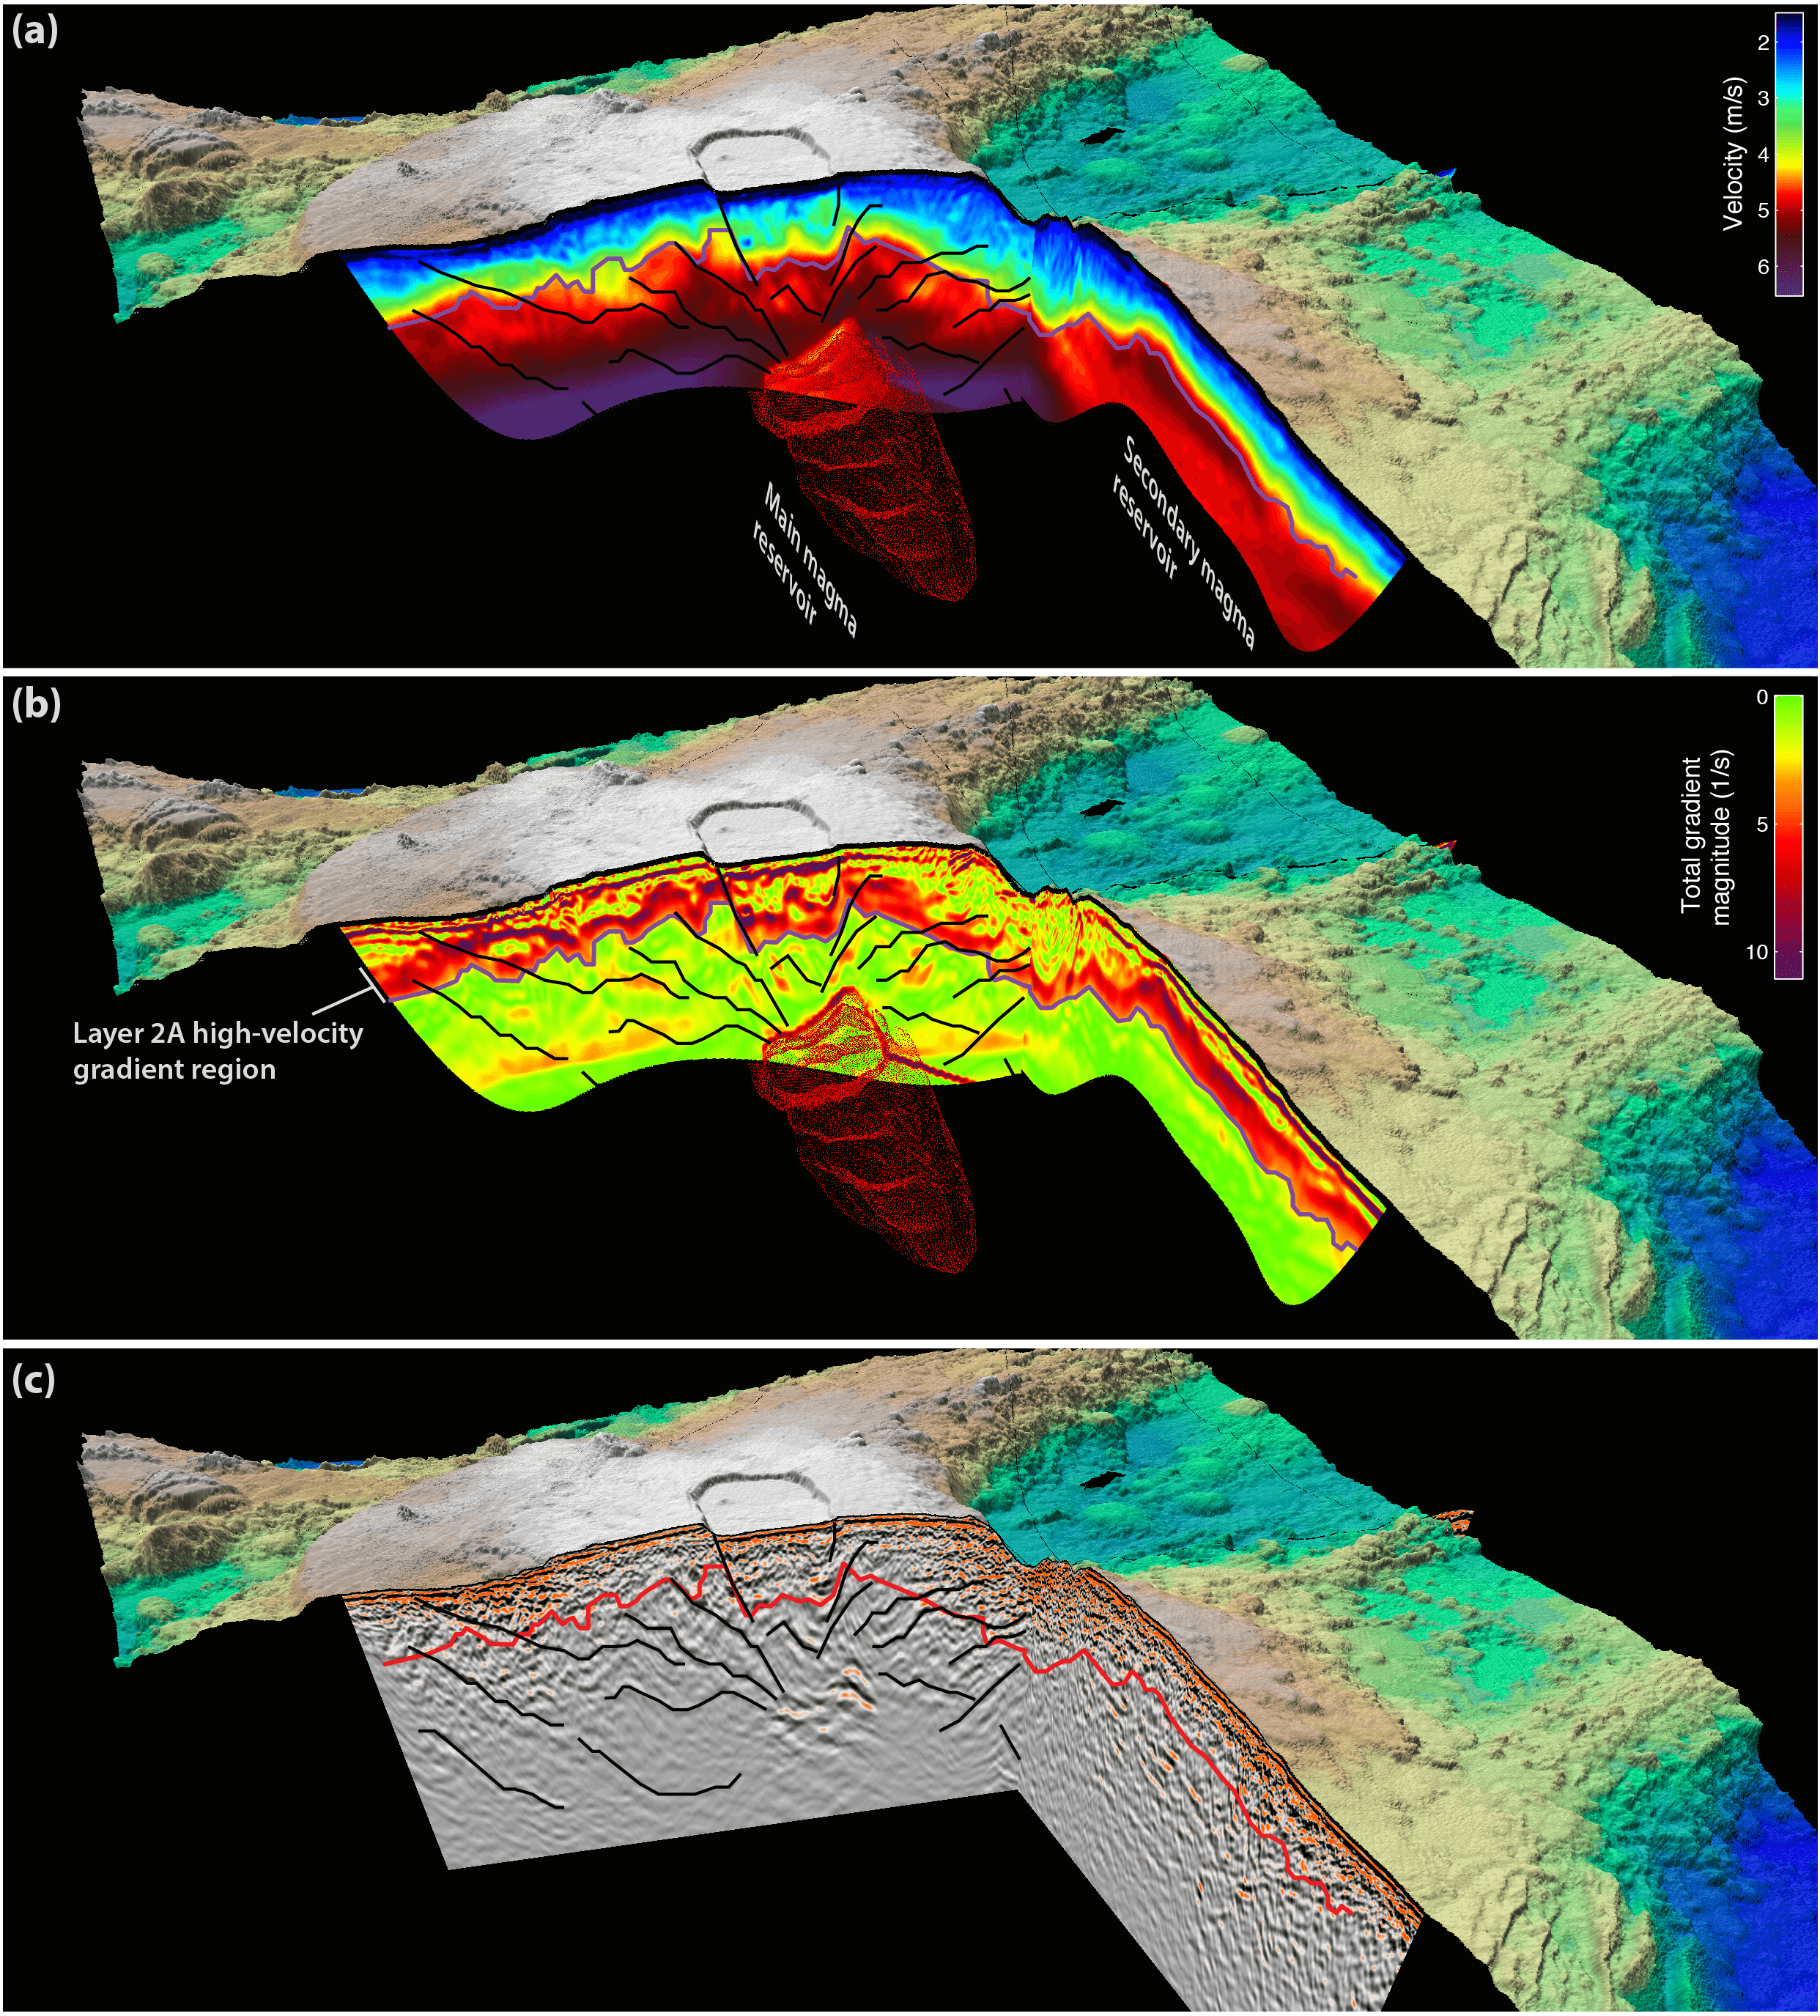
\includegraphics[width=0.75\linewidth]{FWI1.png}
  \caption{Seismic Full Waveform Inversion}
  \label{fig:FWI1}
\end{figure}

In FWI, the aim is to find the media properties on a dense subsurface grid, instead of image amplitudes. Synthetic seismic data are forward modeled and compared with the measured dataset. The differences are then used to update the full set of media properties and the process is repeated until a satisfactory match between modeled and measured dataset is obtained. In Figure \ref{fig:FWI2} \newstm{a} flow chart for the process is shown. It can be seen that, in contrast to imaging techniques, a closed loop exists, meaning that feedback from the obtained media properties is used to verify any inconsistency between the measured data and the inversion result. In the flow chart we can see that we begin with forward modelling and estimate the synthetic data. Further, we iterate the data in order to minimise the residuals as compared to the real data and obtain the final data once the residuals are below the specified tolerance levels.
\commentstm{Show this requirement in the picture}\brok\ IMPLEMENTED.

\begin{figure}
\centering
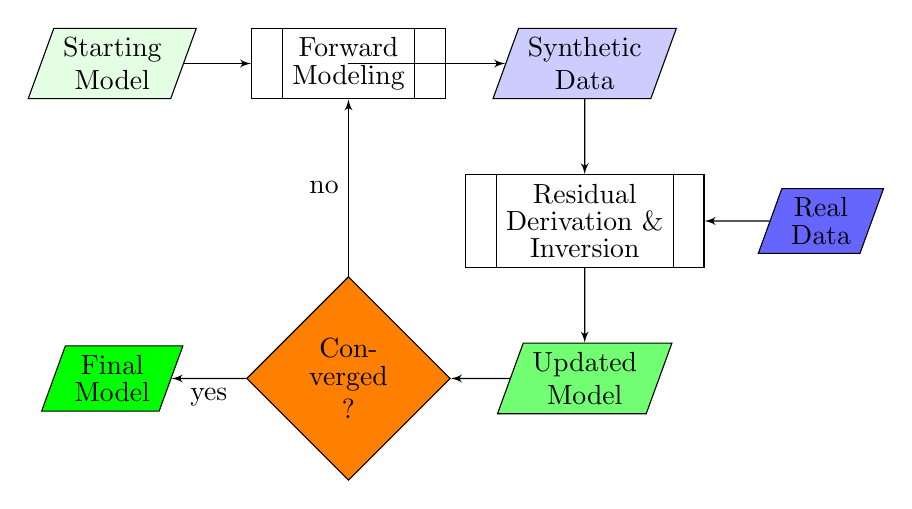
\begin{tikzpicture}[node distance = 2cm, auto]
    \node [draw,rectangle split, rectangle split horizontal,rectangle split parts=3] (init) {\nodepart{two}{\shortstack{Forward\\ Modeling}}};
    \node [draw, trapezium,trapezium left angle=70,trapezium right angle=-70, left of=init, node distance = 3cm, fill=green!10] (expert) {\shortstack{Starting\\ Model}};
    \node [draw, trapezium,trapezium left angle=70,trapezium right angle=-70,right of=init, node distance = 3cm, fill=blue!20] (system) {\shortstack{Synthetic\\ Data}};
    \node [draw, below of=system, rectangle split, rectangle split horizontal,rectangle split parts=3] (identify) {\nodepart{two}{\shortstack{Residual\\ Derivation \& \\ Inversion}}};
        \node [draw, trapezium,trapezium left angle=70,trapezium right angle=-70,right of=identify, node distance = 3cm, fill=blue!60] (new){\shortstack{Real\\ Data}};
    \node [draw, trapezium,trapezium left angle=70,trapezium right angle=-70,below of=identify, fill=green!55] (evaluate) {\shortstack{Updated\\ Model}};
    \node [decision, left of=evaluate, fill=orange] (decide) {\shortstack{Con-\\ verged\\ ?}};
    \node [draw, trapezium,trapezium left angle=70,trapezium right angle=-70,left of=decide, node distance = 3cm, fill=green] (stop) {\shortstack{Final\\ Model}};
    \path [line] (system) -- (identify);
    \path [line] (identify) -- (evaluate);
    \path [line] (evaluate) -- (decide);
    \path [line] (decide) -- node {no}(init);
    \path [line] (decide) -- node {yes}(stop);
    \path [line] (expert) -- (init);
    \path [line] (init)|-(system);
    \path [line] (new)--(identify);
\end{tikzpicture}
\caption{Full Waveform Inversion Methodology\label{FWI2}}
\end{figure}

\begin{comment}
\begin{figure}
  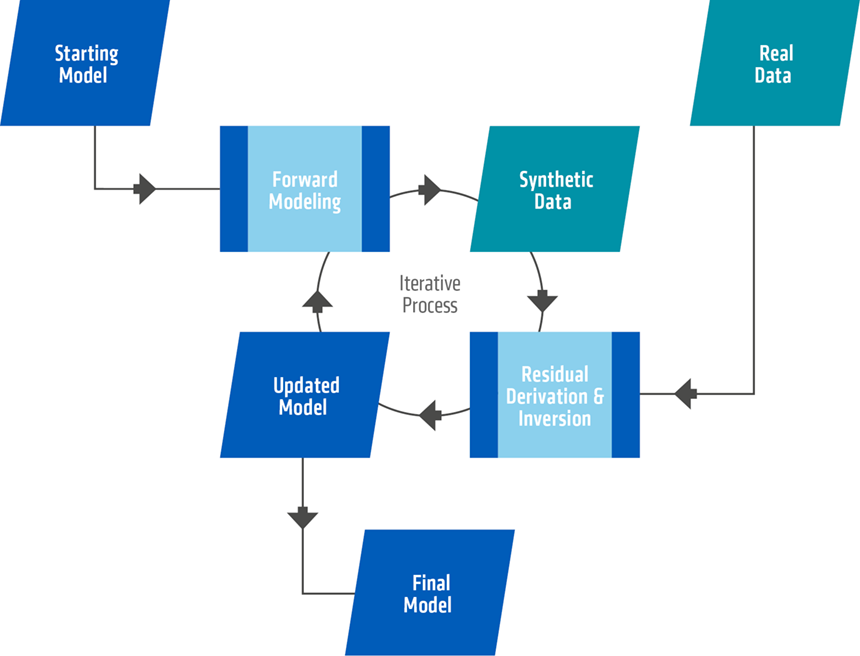
\includegraphics[width=\linewidth]{FWI2.png}
  \caption{Full Waveform Inversion Methodology. \commentstm{Ideally this image would contain what we call a BREAK condition. Does it stop, because a number of iterations has been performed or because the system converged? If it is the first thing, does the system warn clearly that there is no convergence?}}
  \label{fig:FWI2}
\end{figure}
\end{comment}

This document \oldstm{explains}\newstm{provides} an overview of the equations employed, the computational model and the code algorithm.
\commentstm{I may be wrong, but I don't think that is what it does. It provides an overview of ``the model'' - the mathematical equations used - the parallellization (here referred to as ``the model'') and finalize with a description of each individual module in the code (I would not call this ``the code algorithm'' at all myself.)}

\section{Mathematical Model}
\commentbr{For this section, BR prefers to start with eq 5; because G follows from 2, which follows from 5}
The mathematical model outlines the equations used in the code for the FWI.
\commentstm{weird sentence}
We begin with the Green's function and apply it to the \oldstm{the} simplest acoustic equation - the Helmholtz equation.
For the acoustic case with constant density, the wave equation can be described by a set of two couples \commentstm{coupled?} equations, being the data equation and the object equation. The data equation describes the seismic dataset, in terms of a total field $p_{\text{tot}}$ at each grid point in the subsurface, the contrast function $\chi$ and the Green's function $\mathcal{G}$ \commentstmtwo{corrected} in a background medium: \commentstm{It is slightly confusing that the contrast function is defined later unannounced and Green's is provided immediately}

\begin{equation} \label{eq:eq1}
p_\text{data}(\mathbf{x_\text{r}},\mathbf{x_\text{s}},\omega) = \int \mathcal{G}(\xr, \x, \omega) p_\text{tot}(\x, \xs, \omega) \chi(\x) \df{\x} \end{equation}

\newstmtwo{The indices \textbf{s} and \textbf{r} are for ``source'' and ``receiver''} \brok.
Reading from right to left, equation \ref{eq:eq1} can be understood as follows: A source transmits a wavefield that propagates to every point in the subsurface. Note that this wavefield $p_\text{tot}$ is generally quite complex because it takes the interaction of all scatterers in the subsurface already into account. This wavefield is creating secondary sources in all points where the contrast function $\chi$ is non-zero. The secondary sources transmit energy through a smooth background medium to the receivers, represented by the Green's function G in equation \ref{eq:eq1}. \linebreak
\newline
The measured seismic data at every receiver are then a summation of all secondary sources. It should be mentioned that direct waves, including ground roll and surface waves are supposed to be removed from the measured data to obtain $p_\text{data}$.
\commentbr{Not sure if I really understand this.}
\commentstmtwo{Let's discuss at some point on how best to tackle.s}
\newline

We use the 2-D case for the Helmholtz equation. Further, the Green's function is calculated for this equation. The contrast function has to be determined. Further the conjugate scheme is established to determine the error functional.
\newline

Measured seismic data always contains some form of noise, so the inversion process is required to be regularised. Therefore, we extend the conjugate gradient scheme \oldstm{in a way that it contains} \newstm{so as to include} a multiplicative regularisation factor.

\subsection{The Green's function}
A Green's function is the impulse response of an inhomogeneous linear differential equation defined on a domain, with specified initial conditions or boundary conditions.
The Green's function of this equation is defined as the solution $G(\mathbf{x}, \mathbf{y})$, of the equation

\begin{equation} \label{eq:eq2}
[ \nabla^2 G(\mathbf{x}, \mathbf{y}) + k_0^2 G(\mathbf{x}, \mathbf{y}) = -\delta(\mathbf{x} - \mathbf{y}). ]\end{equation}

The solution to (\ref{eq:eq2}) is then given by

\begin{equation} \label{eq:eq3}[ u_\text{ind}(\mathbf{x}) = \int_{\mathbf{y} \in \mathbb{R}^n} G(\mathbf{x}, \mathbf{y}) f_\text{ind}(\mathbf{y}) \df{\mathbf{y}}.\end{equation}

\commentbr{What is ``ind''}
\commentstm{to be determined}
The interesting cases are the 2D and 3D case. We will first \commentstm{only?} focus on the 2D case . The Green's function is then given by

\begin{equation} \label{eq:eq4}[ G(\mathbf{x}, \mathbf{y}) = \frac{\imath}{4} H_0^{(1)}(k_0 \|\mathbf{x} - \mathbf{y}\|) = -\frac{1}{4} Y_0(k_0 \|\mathbf{x} - \mathbf{y}\|) + \frac{\imath}{4} J_0(k_0 \|\mathbf{x} - \mathbf{y}\|).  ]\end{equation}

In the above equation, the $H_0$ , $J_0$ and $Y_0$ are defined as the Henkel's functions and can be further researched at : \url{http://amcm.pcz.pl/get.php?article=2012_1/art_06.pdf}

\subsection{Helmholtz equation}

The simplest model we can use is the acoustic Helmholtz equation. We use a scalar pressure field $u(\mathbf{x})$ and the domain is modeled using $\chi(\mathbf{x})$. and is called the contrast and can be directly related to the wave speed at that point in the domain. Mathematically the equation has the form:

\begin{equation} \label{eq:eq5}
\nabla^2 u(\mathbf{x}) + k(\mathbf{x})^2 u(\mathbf{x}) = -f_{\text{ext}}(\mathbf{x}).
\end{equation}

The wave number $k$ is given by $k = \frac{\omega}{c}$ where $\omega$ is the angular frequency \commentstm{in Hz?}  and c \oldstm{is} the acoustic wave velocity \newstmtwo{in m/s} {\brok} of the true medium.  We split the pressure field into $u(\mathbf{x}) = u_0(\mathbf{x}) + u_{\text{ind}}(\mathbf{x})$, where $u_0(\mathbf{x})$ is defined as the field given by the background velocity and external sources,

\begin{equation} \label{eq:eq6}
\nabla^2 u_0(\mathbf{x}) + k_0^2 u_0(\mathbf{x}) = -f_{\text{ext}}(\mathbf{x}).
\end{equation}

Substituting in (\ref{eq:eq6}) results in

\begin{equation} \label{eq:eq7}
\nabla^2 u_\text{ind}(\mathbf{x}) + k_0^2 u_\text{ind}(\mathbf{x}) = -f_\text{ind}(\mathbf{x}),
\end{equation}

with $f_\text{ind}(\mathbf{x}) = k_0^2 \chi(\mathbf{x}) u(\mathbf{x})$ the induced source term.


\subsection{The Contrast function}

The contrast function is defined as:

\begin{equation} \label{eq:eq8}\chi(\mathbf{x}) = 1 - \left(\frac{c_0(\vec{x})}{c(\vec{x})} \right)^2. \end{equation}

It depends on the difference between a known background medium $c_\text{0}(\vec{x})$ and the true, but unknown, subsurface model $c(\vec{x})$. The total field on the right-hand side in equation \ref{eq:eq1} is dependent on the contrast, because it contains the interaction between all subsurface scatterers. Then it follows that there is a nonlinear relationship between the subsurface properties and the measured seismic data.

Notice that the contrast is generally unknown, and will be approximated using an iterative scheme. During each step the induced source is considered constant and known so we basically solve the same equation as (\ref{eq:eq3}) each step.

\subsection{The Conjugate Gradient Scheme}
\commentbr{Should this be the start of a new chapter?}
\commentstmtwo{Proposal following BR's question to refer to this and the following chapters as a subsection of  NEW 2.2 ``Computational Model'' and to refer to the previous sections as subsections under a 2.1 ``Physical Model'' with current chapter 3 referred to in the future as ``Implementation'' and the main chapter 2 as ``Modelling''.}
In the inversion scheme, we try to minimise the difference between the measured data $p_\text{data}$ and the modelled data that is obtained using the currently best estimate of the contrast function and the fixed total field.

The residual between the measured and modelled data is obtained as:

\begin{equation} \label{eq:eq9} r(\xr, \xs, \omega) = p_{\text{data}}(\xr, \xs, \omega) - \left[\mathcal{K}_\chi \right](\xr, \xs, \omega), \end{equation}

\commentbr{I always found the K symbol confusing}
\commentstmtwo{I have verified that this is the same notation that Haffinger, the person who wrote the Ph.D. thesis on which this manual is based, uses. So I will add a specific reference to that thesis here, where you can find more background on that particular part.}

with

\begin{equation} \label{eq:eq10} \left[\mathcal{K}_\chi \right](\xr, \xs, \omega) = \int \mathcal{G}(\xr, \x, \omega) p_\text{tot}(\x, \xs, \omega) \chi(\x) \df{\x} \end{equation}

a linear operator in $\chi$, and where we adopt the specific notation by Haffinger (Haffinger, Ph.D. thesis 2013, TU Delft) for consistency.
\commentstm{has a subscript been forgotten in the formula above? Here is an example of BR approving this idea and AP disapproving: }
{\brok}
{\apnok}
The error functional is equal to

\begin{equation} \label{eq:eq11} F(\chi) = \eta \int |r(\xr, \xs, \omega)|^2 \df{\mathbf{x}_\text{s}} \df{\xr} \df{\omega},\end{equation}

with

\begin{equation} \label{eq:eq12} \eta^{-1} = \int | p_\text{data}(\xr, \xs, \omega) |^2 \df{\xs} \df{\xr} \df{\omega}, \end{equation}

so that for $\chi = 0$ we have $F = 1$. Notice the implicit dependency on $\chi$.

We want to find a sequence of contrast functions, $\chi^{(n)}(\vec{x}), n = 1,2,...,$ in which error functional decreases with increasing iterations. Therefore, after each iteration the contrast function is updated as:

\begin{equation} \label{eq:eq13} \chi^{(n)}(\vec{x}) =  \chi^{(n-1)}(\vec{x}) + \alpha_n\zeta_n(\vec{x}) \end{equation}

Here, the step size of the update is determined by the parameter $\alpha_n$ while the update directions are conjugate gradient directions given by

\begin{equation} \label{eq:eq14}\zeta_1(\vec{x}) = g_1(\vec{x}) ,\zeta_n(\vec{x}) = g_n(\vec{x}) + \gamma_n\zeta_{n-1}(\vec{x}) \end{equation}

The functional derivative w.r.t. $\chi$ in direction $\mathbf{d}$ of the error functional is equal to
\begin{subequations}
\begin{align}
\partder{F(\mathbf{\chi}, \mathbf{d})}{\mathbf{\chi}} & = \lim_{\epsilon \rightarrow 0} \frac{F(\mathbf{\chi} + \epsilon \mathbf{d}) - F(\mathbf{\chi})}{\epsilon} \\
& = -2 \eta \int \real{\left[\mathcal{K}_\mathbf{d} \right](\xr, \xs, \omega)^{\dagger} r (\xr, \xs, \omega)} \df{\xs} \df{\xr} \df{\omega}
\label{eq:hi}
\end{align}
\end{subequations}

\newstmtwo{The derivation of this equation is provided in section \ref{deriveerrorfunctional}.}
{\brok}

For the discrete $\mathcal{K}$ operator the integrand will have the form

\begin{equation} \label{eq:eq15} g_n(\vec{x}) = \eta \real{[\mathcal{K}^\star\mathbf{r}_{n-1}](\vec{x})} \end{equation}

where the $\star$ denote element wise multiplication per row and Re denotes that only the real part will be used.
The adjoint operator $[\mathcal{K}^\star\mathbf{r}_{n-1}]$ can be seen as a backprojection operator that maps the residual between measured data and modelled data from the surface domain to its associated location in the scattering domain.

In our conjugate gradient scheme we make use of the Polak-Ribi$\grave{e}$re direction,

\begin{equation} \label{eq:eq16} \gamma_n = \frac{\int g_n(\vec{x})[g_n(\vec{x})-g_{n-1}(\vec{x})]d(\vec{x})}{\int g_{n-1}(\vec{x}) g_{n-1}(\vec{x})d(\vec{x})} \end{equation}

The optimal step size is found from the minimisation of cost functional equation, by setting the derivative equal to zero. Consequently the optimal step size becomes:

\begin{equation} \label{eq:eq17} \alpha_n = \frac {\real {\int \int \int r^{\star}_{n-1}(\mathbf{x_\text{r}},\mathbf{x_\text{s}},\omega)[\mathcal{K} \zeta_n](\mathbf{x_\text{r}},\mathbf{x_\text{s}},\omega)d\vec{x_s}d\vec{x_r}d\omega}}{\int \int \int \mid[\mathcal{K} \zeta_n](\mathbf{x_\text{r}},\mathbf{x_\text{s}},\omega) \mid^2 d\vec{x_s}d\vec{x_r}d\omega} \end{equation}

To initialise the conjugate gradient scheme, we assume, $\chi^0 (\vec{x}) = 0$, leading to $r_0(\mathbf{x_\text{r}},\mathbf{x_\text{s}},\omega) = p_{data}(\mathbf{x_\text{r}},\mathbf{x_\text{s}},\omega)$.
\commentstmtwo{correction of superscript}
Therefore, we find the gradient as :

\begin{equation} \label{eq:eq18} g_1(\vec{x}) = \eta \real{[\mathcal{K}^\star p_\text{data}](\vec{x})} \end{equation}

and we get the first update parameter as :

\begin{equation} \label{eq:eq19} \alpha_1 = \frac {\real {\int \int \int p^{\star}_\text{data}(\mathbf{x_\text{r}},\mathbf{x_\text{s}},\omega)[\mathcal{K} g_1](\mathbf{x_\text{r}},\mathbf{x_\text{s}},\omega)d\vec{x_s}d\vec{x_r}d\omega}}{\int \int \int \mid[\mathcal{K} g_1](\mathbf{x_\text{r}},\mathbf{x_\text{s}},\omega) \mid^2 d\vec{x_s}d\vec{x_r}d\omega} \end{equation}


\subsection{Multiplicative Regularisation}

Since all seismic data contains some form of noise, the inversion process needs to be stabilised. Therefore, the CG scheme is extended in a way that it contains a multiplicative regularisation factor.

The error functional $\mathcal{F}^{tot}$ becomes a product of the original error functional and a newly introduced regularisation factor $\mathcal{F}^{reg}$:

\begin{equation} \label{eq:eq20} \mathcal{F}^{tot}_n = \mathcal{F}^{data}_n \mathcal{F}^{reg}_n \end{equation}

The following weighting function is used:

\begin{equation} \label{eq:eq21} b_n^{2} = (\int_{\vec{x}} d\vec{x})^{-1} (\mid\nabla\chi^{n-1}\mid^2 + \delta_{n-1}^2)^{-1} \end{equation}

In the above equation, the $\delta_{n}^2$ is the steering factor and can be defined as:

\begin{equation} \label{eq:eq22} \delta_{n}^2 = (\int_{\vec{x}} d\vec{x})^{-1} \int_{\vec{x}} \mid\nabla\chi^{n-1}\mid^2 d\vec{x} \end{equation}

The new total cost functional then becomes a \oldstmtwo{sum}\newstmtwo{product} {\brok} of two second order polynomials:

\begin{equation} \label{eq:eq23} \mathcal{F}^{tot}_n = (\mathcal{A}_2\alpha^{2}_n + \mathcal{A}_1\alpha_n +\mathcal{A}_0)(\mathcal{B}_2\alpha^{2}_n + \mathcal{B}_1\alpha_n + \mathcal{B}_0) \end{equation}

\oldstm{in which the constants are given by:}
%\commentstm{There used to be equations here and now not anymore.}
\newstmtwo{with the constants A\textsubscript{0}, ..., A\textsubscript{2}, B\textsubscript{2} in appendix \ref{totalcostprefactors}} {\brok}

\subsection{Nonlinear field update based on the domain equation}

Initially, the subsurface properties are unknown  and the very first inversion is based on the assumption that wavefield propagation occurs in smooth non-scattering background medium only.
\commentstm{I would like to know whether that is really the only assumption we are making and whether it should be referred to as an assumption or a first guess}
Using an approximate smooth property model of the subsurface immediately tells us that the wavefield propagation in such an approximate medium cannot be exact \commentstm{When I think of ``exact'' I think of an exact solution to an equation, not to a highly accurate result. Should it be ``accurate''?} and that for exact results we should make the wavefields consistent with the currently best estimate of the true medium. For this reason we assume $p_{tot} \approx p_0$.

Since the output of linear full waveform inversion is a property model, we do
not only obtain structural information but also a first order approximation of the subsurface properties at every grid point in the inversion domain. We can now use this property model to update the total field by solving the domain equation with in principle any suitable numerical method. Therefore, we iteratively build up the total fields as a sum of the background field and a number of basis functions:

\begin{equation} \label{eq:eq30} \phi_n (\mathbf{x_\text{r}},\mathbf{x_\text{s}},\omega) = \int_{\vec{x}\in D} \mathcal{G} (\mathbf{x_\text{r}},\mathbf{x_\text{s}},\omega)\partial \mathcal{W}_n d\vec{x}' \end{equation}

And the incremental contrast sources $\partial \mathcal{W}_n$ are given by:

\begin{equation} \label{eq:eq31} \partial \mathcal{W}_1 = \chi^{(1)} p^{0}_{tot} , \mathcal{W}_n = \chi^{(n)} p^{n-1}_{tot} - \chi^{(n-1)} p^{n-2}_{tot}, n > 1. \end{equation}

The weighting factors are then determined and $p_tot$ is updated according to the equation:

\begin{equation} \label{eq:eq32} p^{(N)}_{tot} (\mathbf{x_\text{r}},\mathbf{x_\text{s}},\omega) =  p_0 (\mathbf{x_\text{r}},\mathbf{x_\text{s}},\omega) + \sum\limits_{N=1}^N \alpha^{(N)}_n (\mathbf{x_\text{s}},\omega) \phi_n (\mathbf{x_\text{r}},\mathbf{x_\text{s}},\omega) \end{equation}

\section{Computational Model}
\commentstm{Feels like this section, and the way we refer to it, is ``Parallellization of the Computations: from a single CPU to multiple.''}
The message passing interface (MPI) is a standardized means of exchanging messages between multiple computers running a parallel program across distributed memory.

In parallel computing, multiple computers - or even multiple processor cores within the same computer - are called nodes.  Each node in the parallel arrangement typically works on a portion of the overall computing problem. The challenge then is to synchronize the actions of each parallel node, exchange data between nodes and provide command and control over the entire parallel cluster. The message passing interface defines a standard suite of functions for these tasks.

For the FWI, the user sets in the input parameters, if GPU or CPU should be used. This is already checked in the beginning of the code and the appropriate functions corresponding to each are used. Further, the user also sets whether the frequency distribution should be group or alternate. This means that instead of splitting calculations over frequency chunks, split them alternatively over frequency for a better load balancing.


\section{Code Algorithm}
\commentstm{This section sounds more like the manual for each individual module of the code.}
The Code Algorithm is complicated and can be divided into the mathematical functions and the computational functions.

For the mathematical functions, please refer to the \texttt{FWI.vpp}. It explains the \texttt{main.cpp} and the classes defined for this project. The main function basically creates the objects required for the inversion and then called the inversion \texttt{cpu.h} function which performs the main tasks. A high level representation of the \texttt{main.cpp} can be seen in Figure \ref{fig:fig3}.

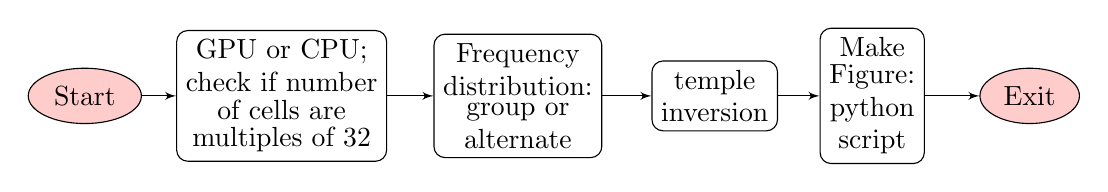
\begin{tikzpicture}[node distance = 3.0cm, auto]
%\begin{tikzpicture}
    \node [cloud] (start) {\shortstack{Start}};
    \node [rectangle, draw,
    text centered, rounded corners, right of=start, node distance = 2.5cm] (processors) {\shortstack{GPU or CPU; \\ check if number \\ of cells are \\ multiples of 32}};
    \node [rectangle, draw,
   text centered, rounded corners, right of=processors, node distance = 3.0cm] (freqdist) {\shortstack{Frequency\\ distribution:\\ group or\\ alternate}};
   \node [rectangle, draw,
   text centered, rounded corners, right of=freqdist,node distance = 2.5cm] (tempinv) {\shortstack{temple\\ inversion}};
   \node [rectangle, draw,
   text centered, rounded corners, right of=tempinv, node distance = 2.0cm] (python) {\shortstack{Make\\ Figure: \\ python\\ script}};
   \node [cloud, right of=python, node distance = 2.0cm] (exit) {\shortstack{Exit}};

    \path [line] (start) -- (processors);
    \path [line] (processors) -- (freqdist);
    \path [line] (freqdist) -- (tempinv);
    \path [line] (tempinv) -- (python);
    \path [line] (python) -- (exit);
\end{tikzpicture}

\begin{figure}
\centering
 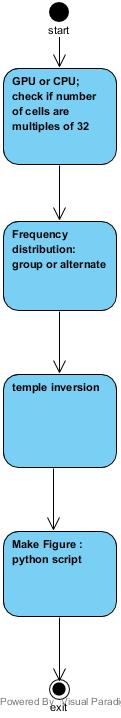
\includegraphics[scale=0.75]{main.jpg}
  \caption{High Level activity diagream for main.cpp}
  \label{fig:fig3}
\end{figure}


\subsection{Input parameters}
\commentstm{I always use the ``courier'' / `texttt'' font to highlight real code stuff among text. I find it extremely pleasant to look at and see other people do it too. It distinguishes code from text and I did it here.}
The input parameters can be defined by running the GUI.py file. It generates a GUI where input parameters can be set.

The inputs for the program are as follows:
\begin{enumerate}
    \item \texttt{int nxt}: No. of cells in x (needs to be a multiple of 32 for GPU)
    \item \texttt{int nzt}: No. of cells in y (needs to be a multiple of 32 for GPU)
    \item \texttt{int nSrct}: No. of sources and receivers
    \item \texttt{int nFreq\_Total}: No. of Frequencies
    \item \texttt{int calc\_alpha}: 1 to calculate alpha in CG scheme, 0 otherwise
    \item \texttt{int n\_max}: Max outer loop iterations
    \item \texttt{int n\_iter1}: Max iterations for conjugate gradient scheme
    \item \texttt{int n\_iter2}: Max p\_total iterations
    \item \texttt{int do\_reg}: Perform the multiplicative Regularization
    \item \texttt{double F\_min1}: Minimum Frequency
    \item \texttt{double F\_max1}: Maximum Frequency
    \item \texttt{int freq\_dist\_group}: 1 for group distribution of frequency, 0 for alternate distribution
    \item \texttt{int nFreq\_input}: number of frequencies per processor
    \item\texttt{int gpu}: 1 for GPU, otherwise 0 for CPU
\end{enumerate}

\subsection{\texttt{main.cpp}}

A high level representation of the \texttt{main.cpp} can be viewed in the \texttt{FWI.vpp} as a UML diagram.
\newline

The main.cpp initialises the MPI functions responsible for parallel computations. Frequency distribution group and alternate are determined here and depending on the user input, the objects are created. Further, the main function creates the objects for the temple inversion and calls the appropriate functions as seen in FWI\_temple.

\subsection{\texttt{temple\_inversion}}

The main part of the code can be seen in the \texttt{temple\_inversion}. Over here, the Green's functions and created and the mathematical model detailed in section 2 is executed. A brief explanation of the functions can be seen as follows:

\subsubsection{\texttt{createGreens()}}

This function creates an array of Green's functions of the  Helmholtz equations. It is called from the Inversion class and refers to the equation \ref{eq:eq7}

\subsubsection{\texttt{CreateP0()}}
$p_0$ is the field calculated with the known contrast and due to the explanation given in section 2.6

\subsubsection{\texttt{createTotalField()}}

After the initial approximation, first iterative $p_{tot}$ is calculated here. This is done by calling the function calcfield(). In this function, the equations defined in section 2.5 are calculated. At first the incremental contrast sources are defined according to equation \ref{eq:eq31} and then the $\phi_n$ is constructed. Based on this \ref{eq:eq32} is constructed. This step concludes the forward modelling step.
\newline

Based on the input parameters, \oldstm{alpha}\newstm{$\alpha$} is used if \oldstm{alpha}\newstm{$\alpha$} is 1 and is not used if it is set to 0.

\subsubsection{\texttt{calculateData()}}
Once the total field $p_{tot}$ is obtained, the $p_{data}$ is calculated according to \ref{eq:eq1}.

\subsubsection{\texttt{Reconstruct()}}
The reconstruct function might be the most important function of the code. The code runs in an iterative loop to minimise the residuals. According to tolerance values determined by the user and the max number of iterations, the residuals are minimised in order to obtain $p_{data}$. Once the residuals are minimised below the tolerance level, the final model is obtained.
\newline

The Conjugate Gradient scheme detailed in section 2.4 is coded here.

\subsubsection{\texttt{MakeFigure()}}

Finally, the \texttt{MakeFigure()} function is called which calls a python script to generate the figures.

\section{How to use the FWI}

This section details a step by step process to use the FWI.


The development tools that need to be installed are:
\begin{enumerate}
    \item \texttt{sudo apt-get install git}  $\backslash\backslash$For checking out the repositories
    \item \texttt{sudo apt-get install qt5-default}  $\backslash\backslash$For QtCreator and qmake reuired for building
    \item \texttt{sudo apt-get install g++ }  $\backslash\backslash$Required for compiling
    \item \texttt{sudo apt-get install mpich}  $\backslash\backslash$Needed during Qmake
\end{enumerate}

For the OpenCL:
\begin{enumerate}
    \item \texttt{sudo apt-get install opencl-headers}
    \item \texttt{sudo apt-get install ocl-icd-libopencl1}
    \item \texttt{sudo apt-get install ocl-icd-opencl-dev}
\end{enumerate}


For the Eigen libraries:
\begin{enumerate}
    \item \texttt{sudo apt-get install libeigen3-dev}
\end{enumerate}


For the MakeFigure function and GUI:

\begin{enumerate}
    \item \texttt{sudo apt-get install python2.7-dev}
    \item \texttt{sudo apt-get install python2.7}
    \item \texttt{sudo apt-get install python-tk}
    \item \texttt{sudo apt-get install python-numpy}
    \item \texttt{sudo apt-get install python-matplotlib}
\end{enumerate}

Next, the repository needs to be checked out:
\newline

\texttt{git clone -o redmine https://git.alten.nl/parallelized-fwi.git}
\newline
\texttt{git checkout docs-libraires-getting-started}
\newline

Further, to build the project, first create a folder titled build-try\_qt-Desktop-Release and then:
\newline

\texttt{mkdir Build}
\newline
\texttt{cd Build}
\newline
\texttt{qmake ../}
\newline
\texttt{make -j4}
\newline
\texttt{try\_qt.pro}

\section{Results and Analysis}

The example chosen for the FWI code is the logo of the Delphi \oldstm{reserah}\newstm{research} consortium. The logo includes a greek temple consisting of four major
pillars under a triangularly shaped roof, as shown in Figure \ref{fig:fig4}.
Additionally we added a layer below the temple to represent the basement. The whole structure is embedded in a homogeneous background with a constant acoustic velocity of c = 2000 m/s. The temple and the basement have a constant velocity.
\commentstm{This sentence is strange.}
The Results obtained from running the FWI code can be seen in the following figures:
\commentstm{I would personally explain well which specific settings yield to the particular results presented here.}

\begin{figure}
\centering
 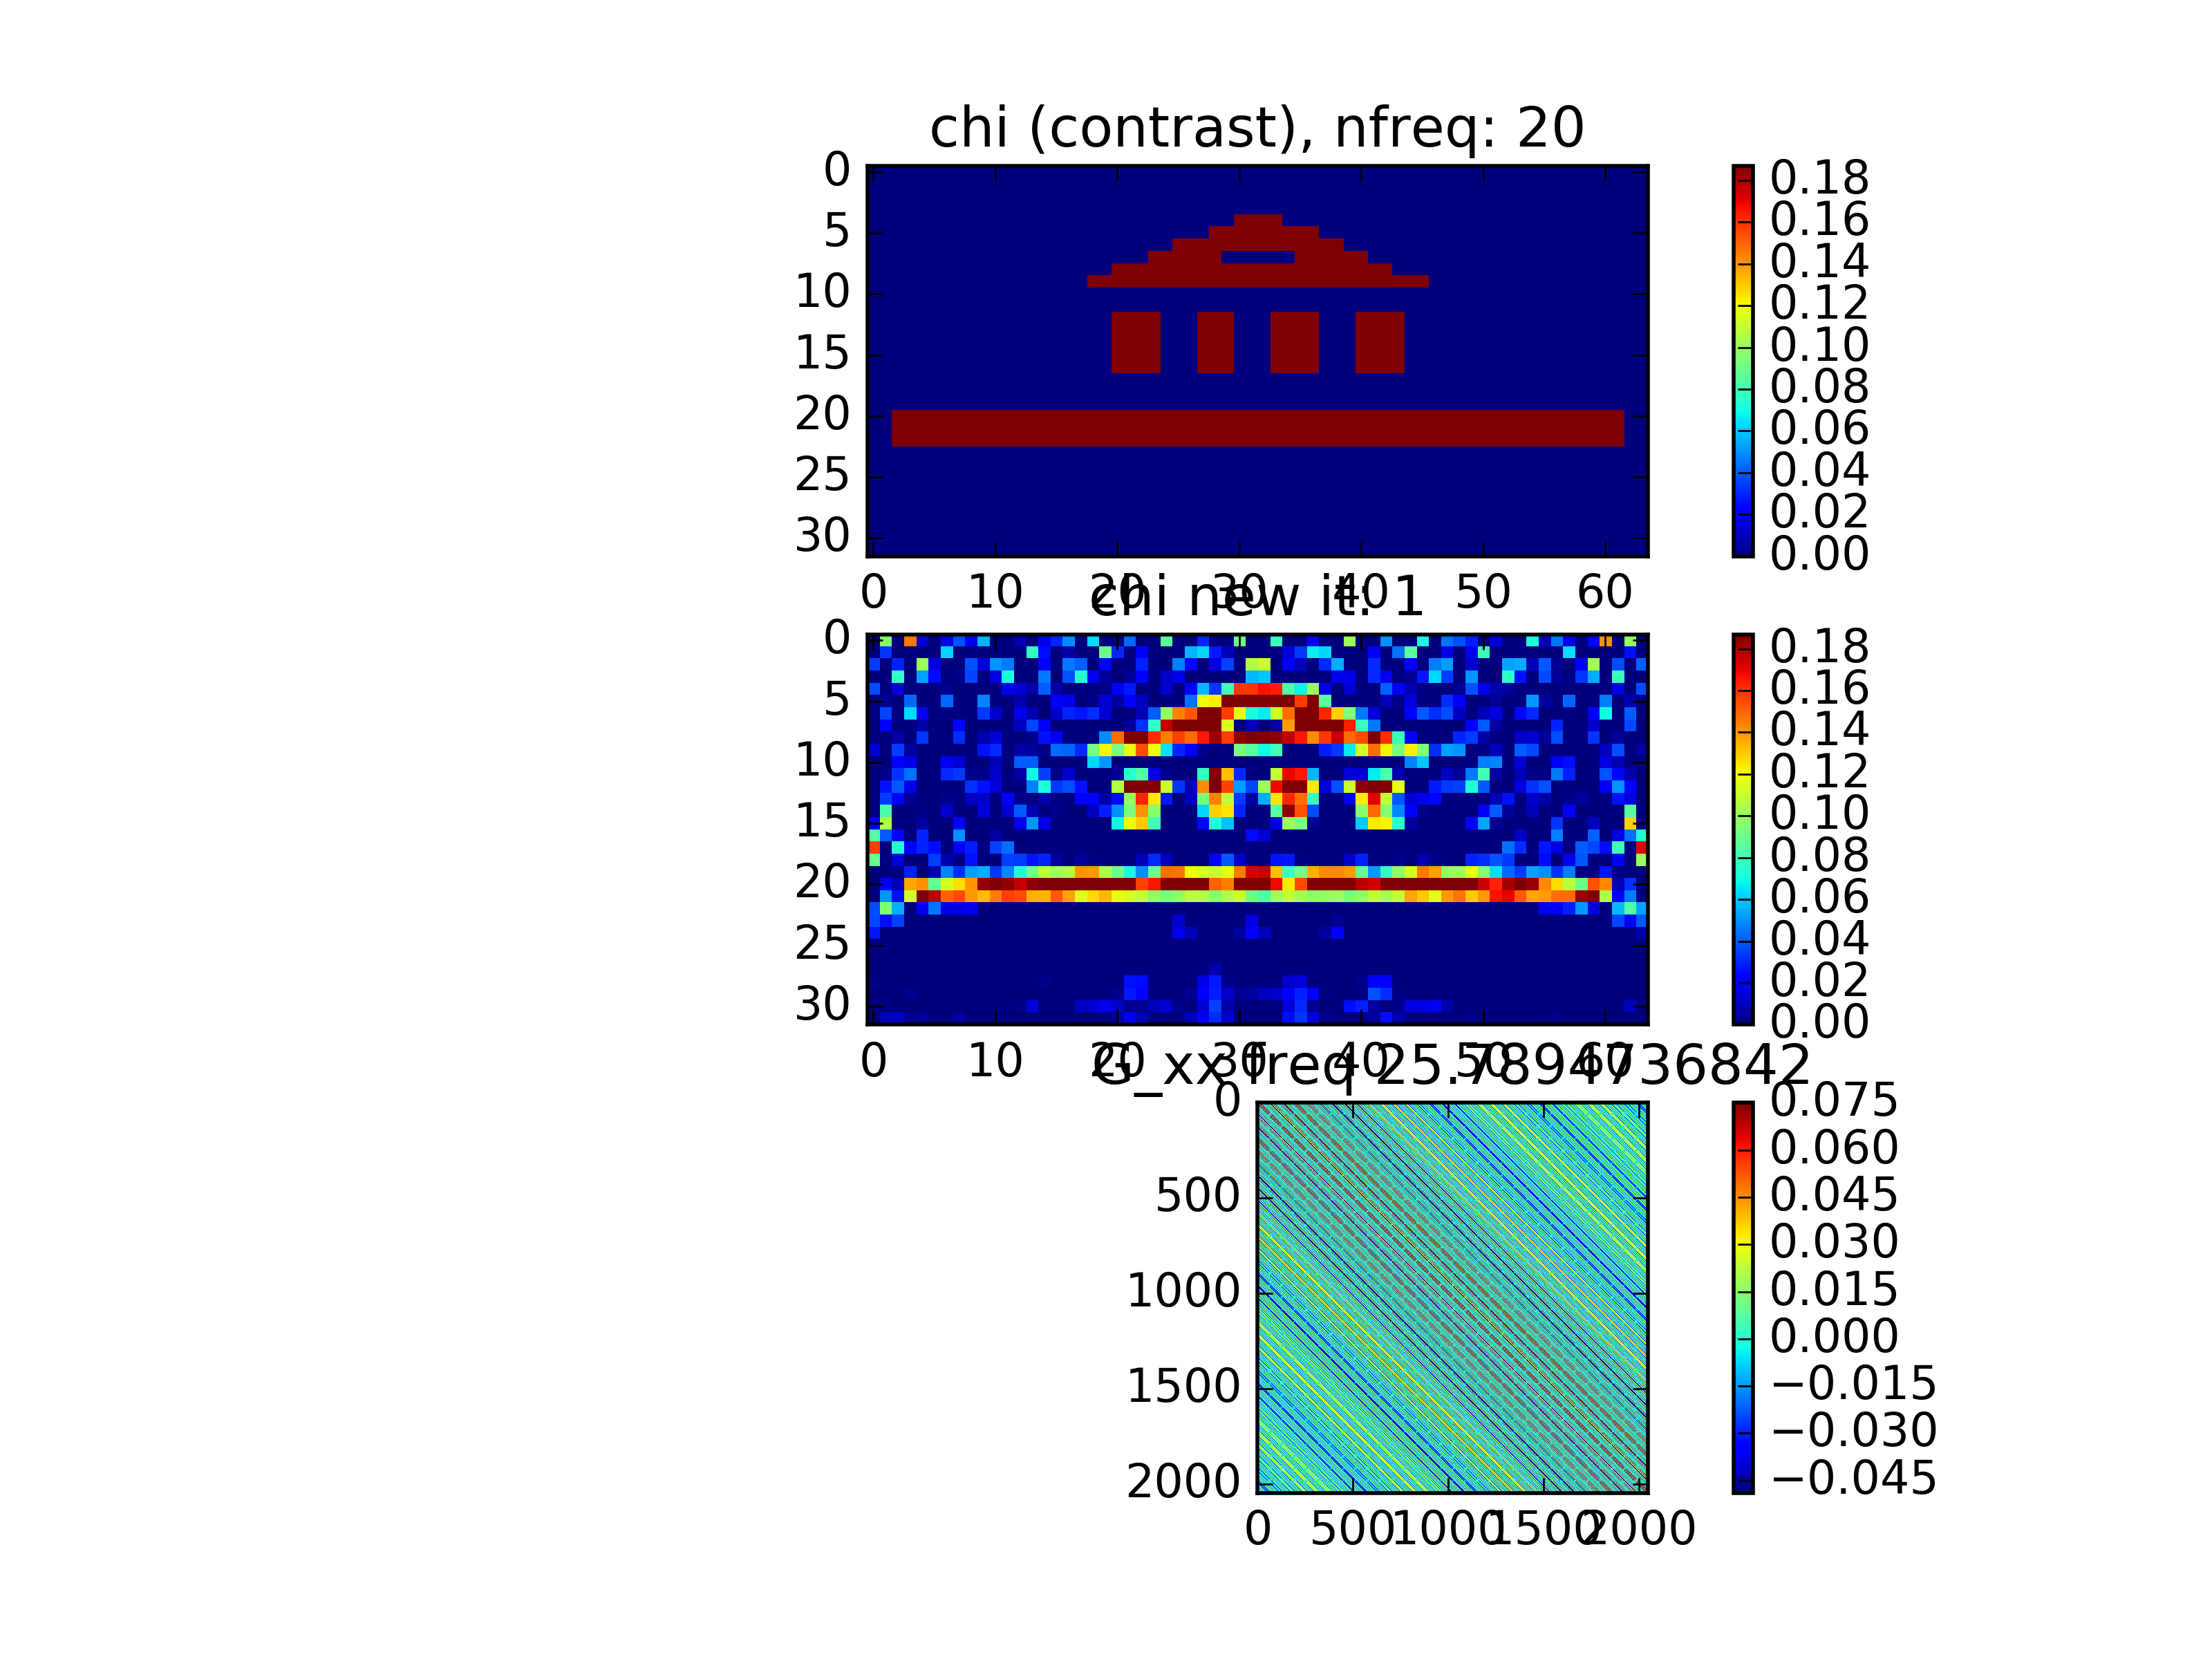
\includegraphics[scale=0.75]{Chi_est_it00.png}
  \caption{Chi estimation Result 1}
  \label{fig:fig4}
 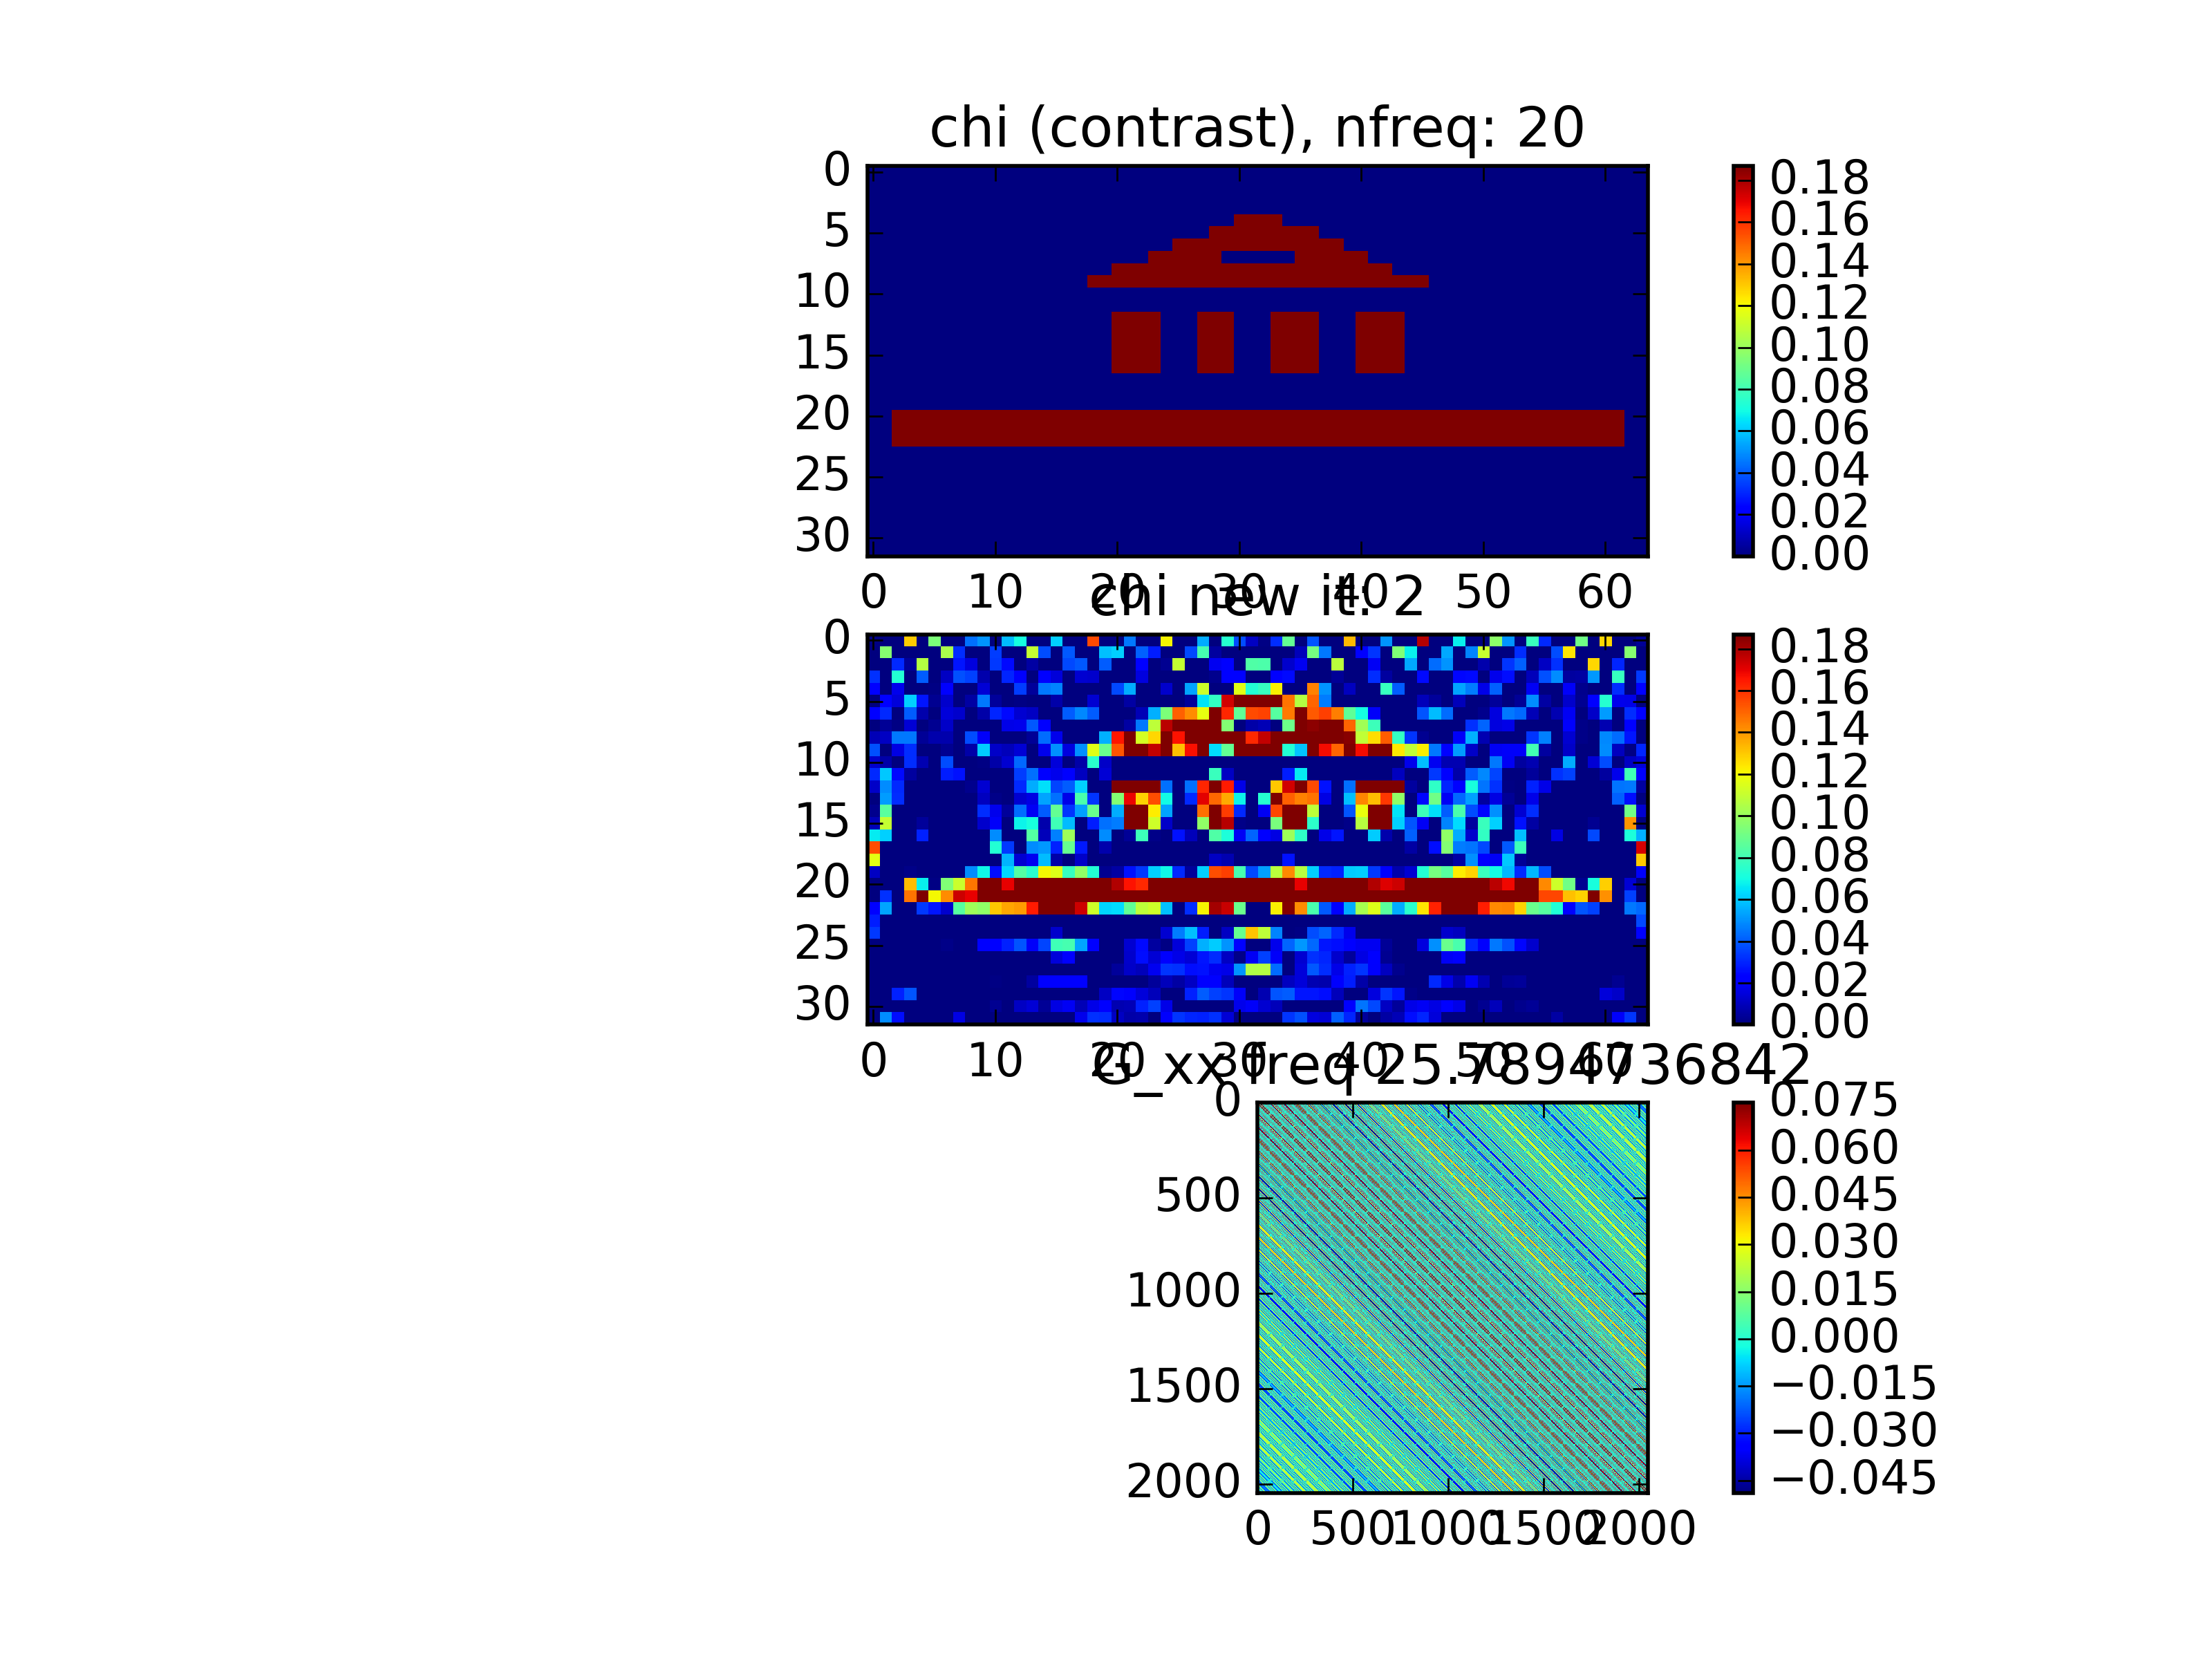
\includegraphics[scale=0.75]{Chi_est_it01.png}
  \caption{Chi estimation Result 2}
  \label{fig:fig5}
\end{figure}

\begin{figure}
\centering
 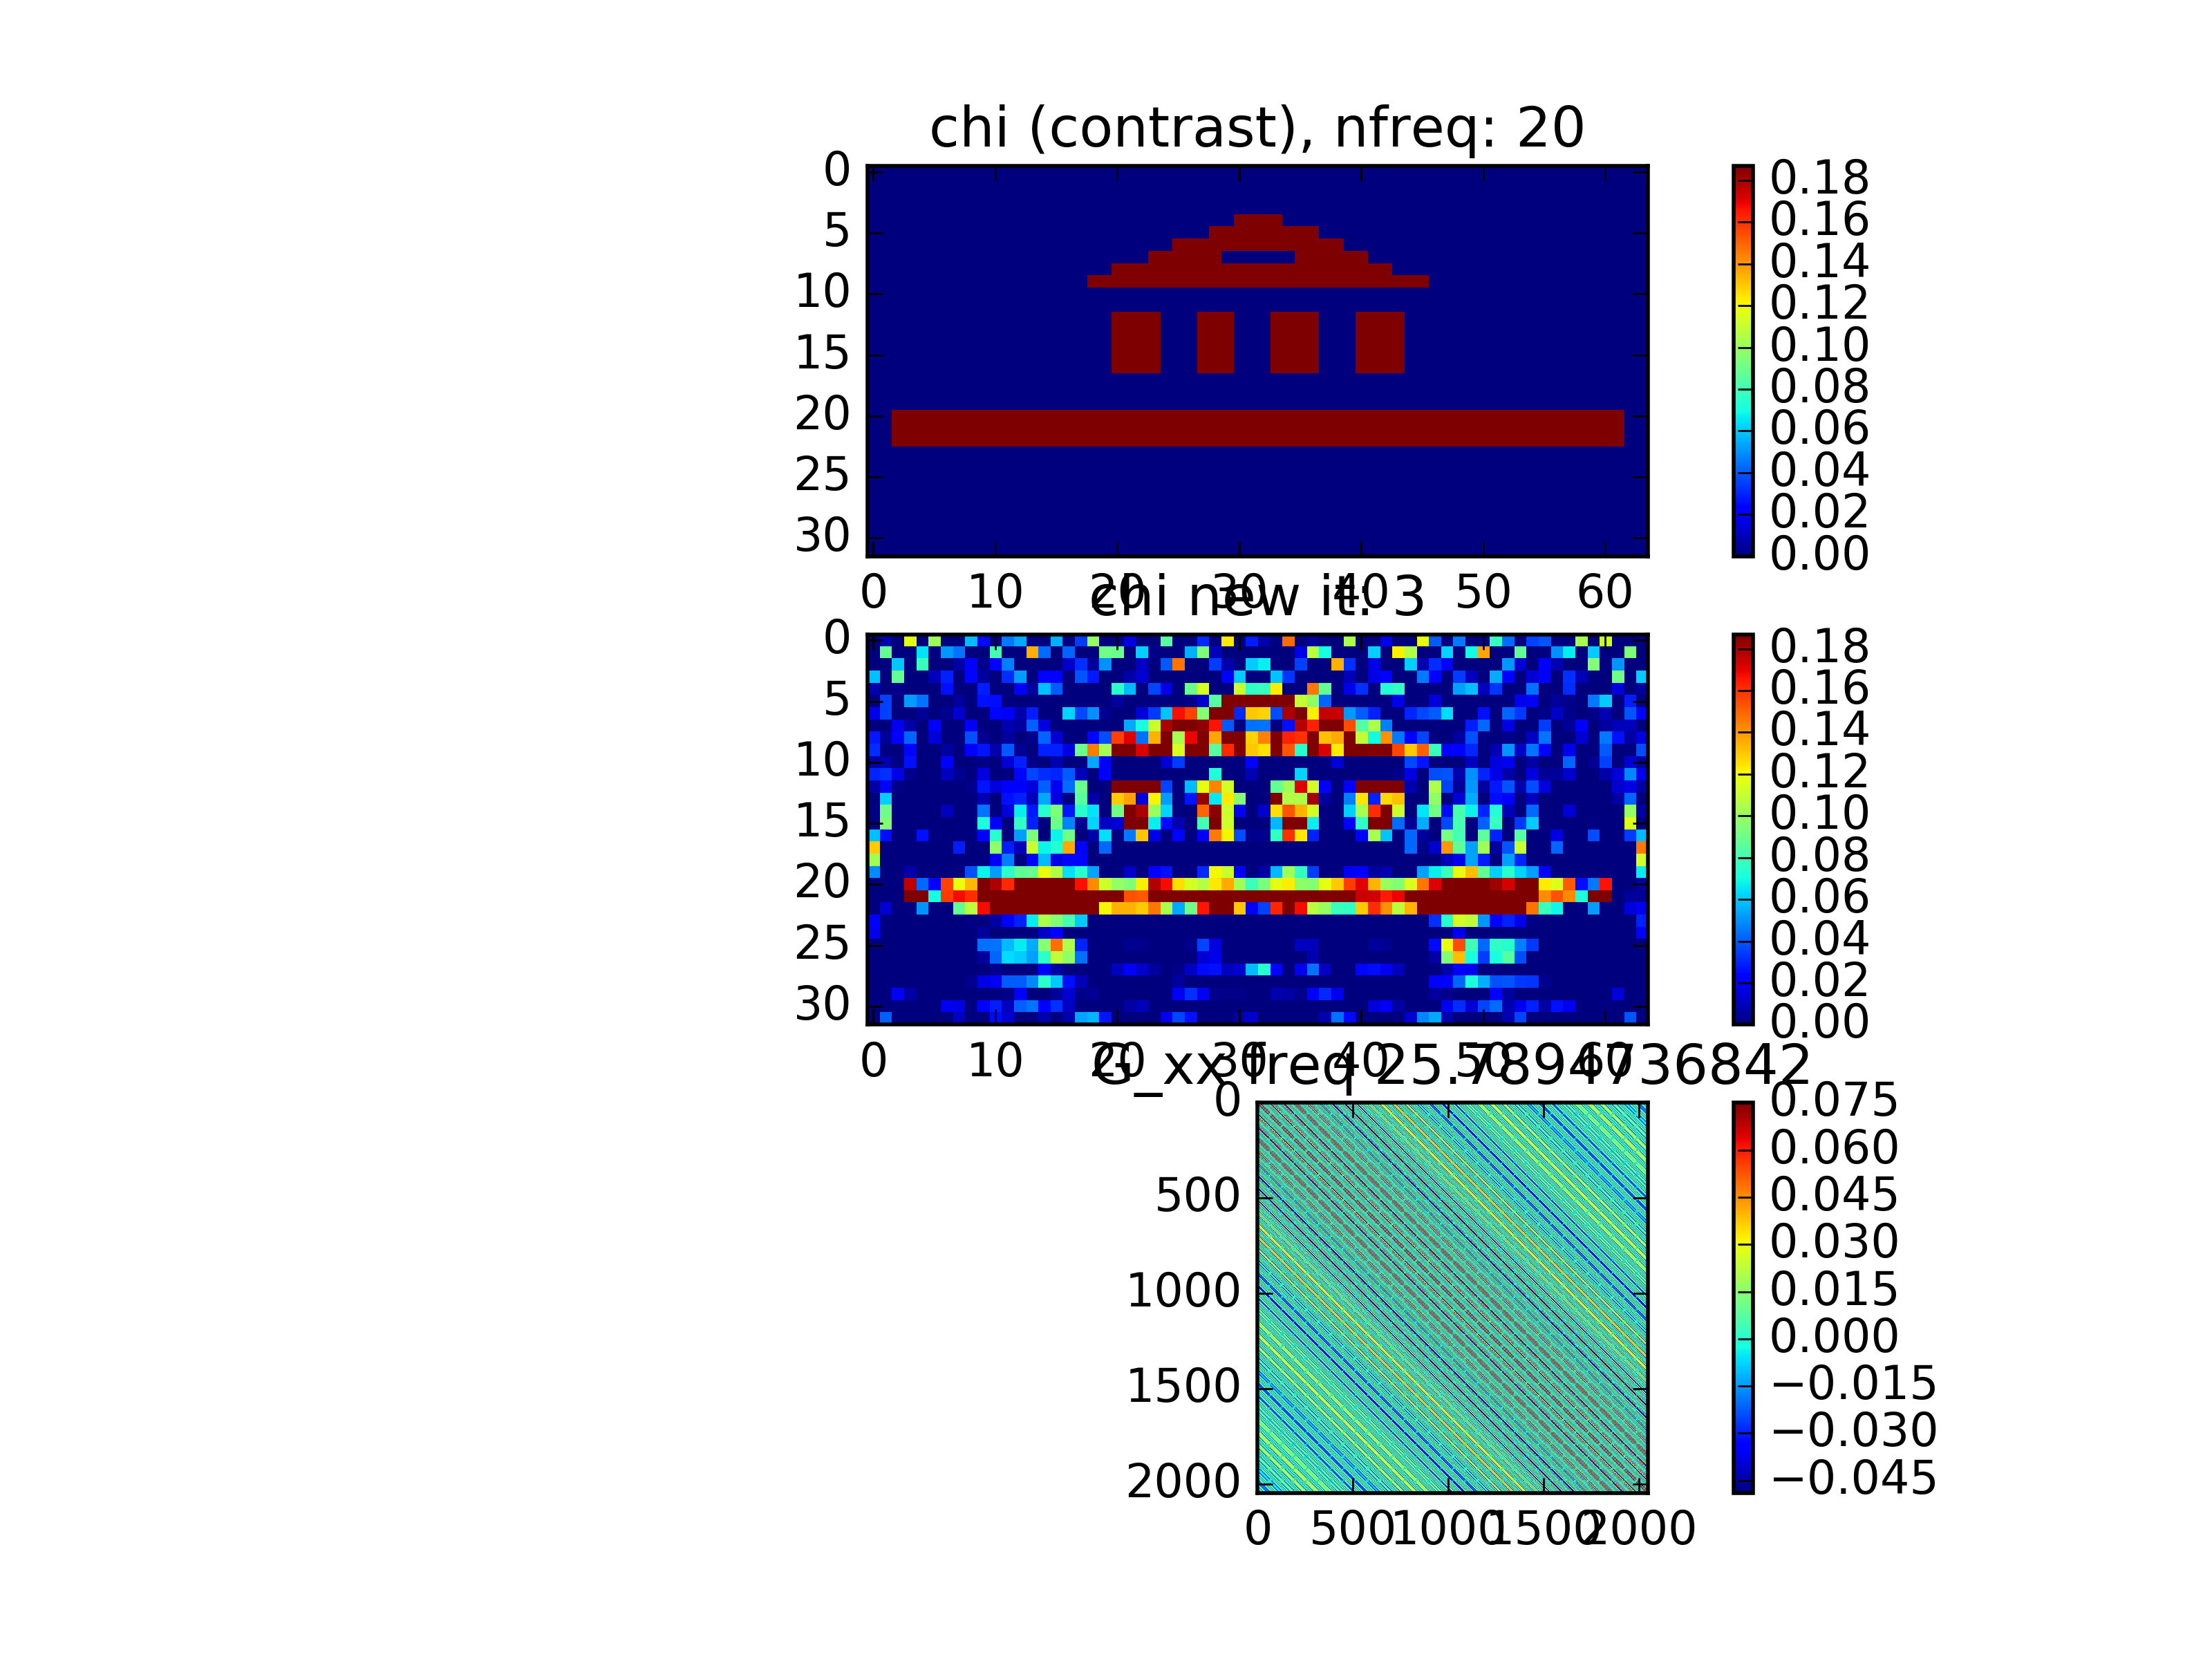
\includegraphics[scale=0.75]{Chi_est_it02.png}
  \caption{Chi estimation Result 3}
  \label{fig:fig6}
 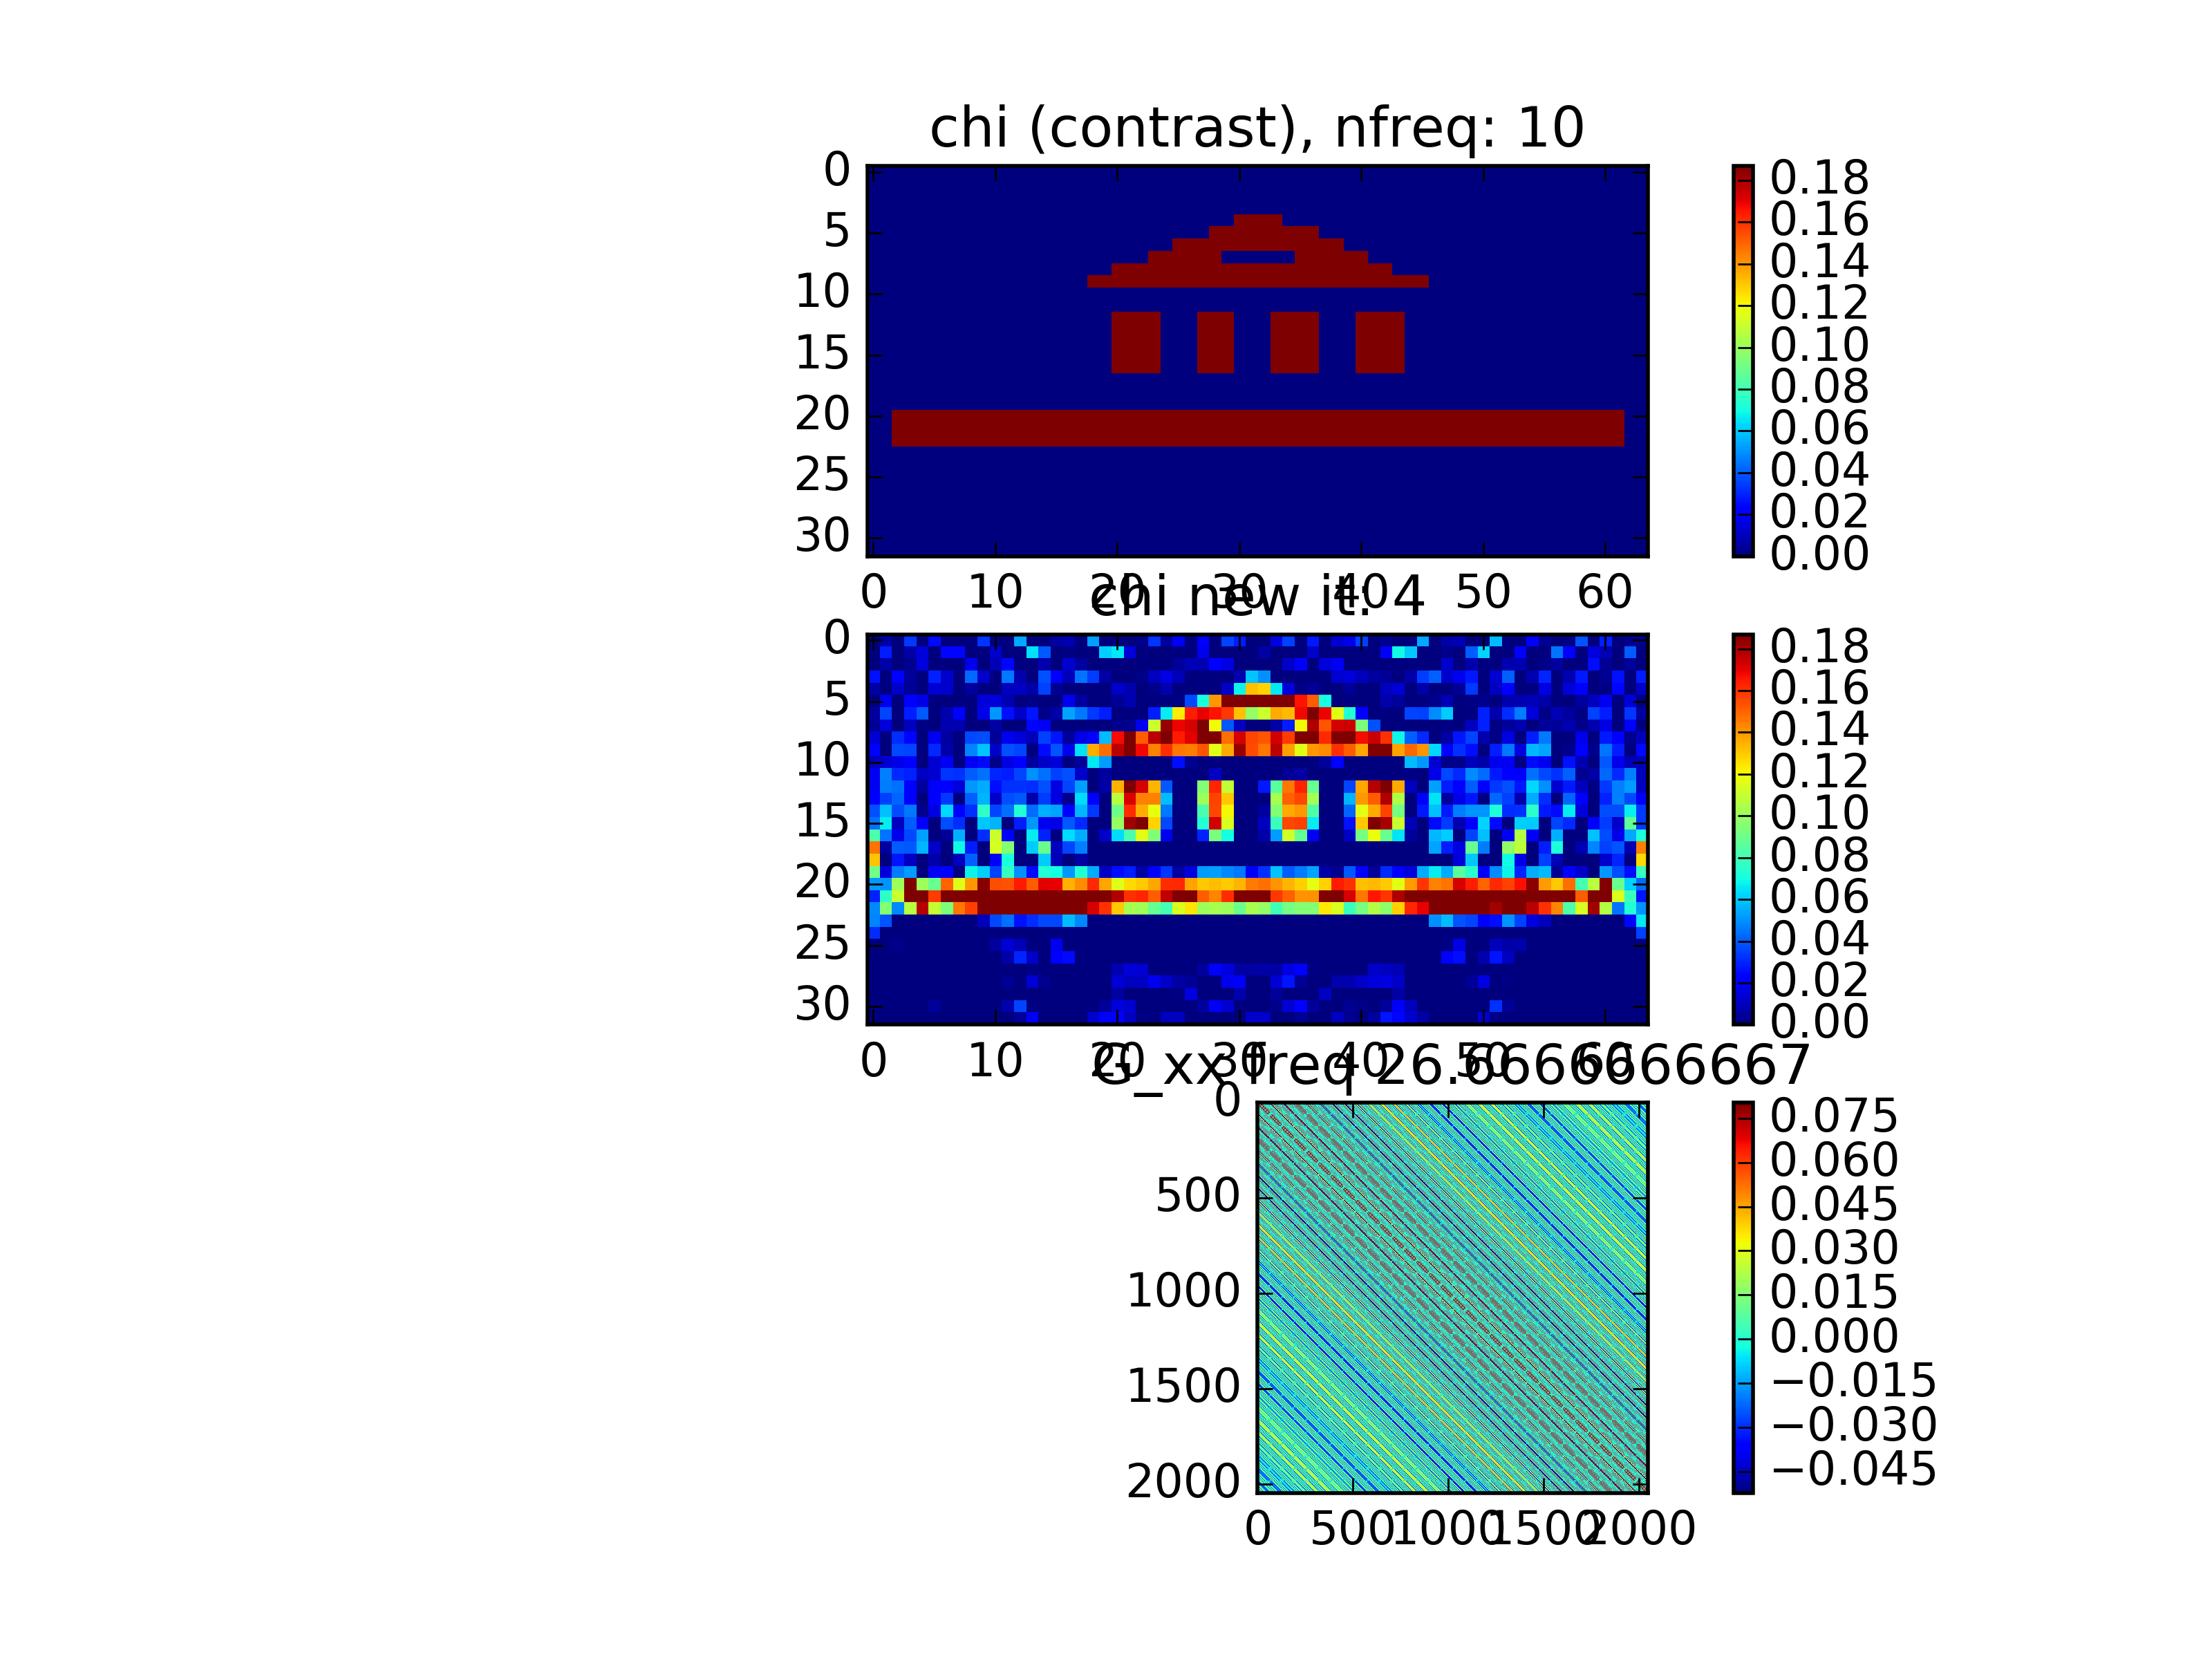
\includegraphics[scale=0.75]{Chi_est_it03.png}
  \caption{Chi estimation Result 4}
  \label{fig:fig7}
\end{figure}

\begin{figure}
\centering
 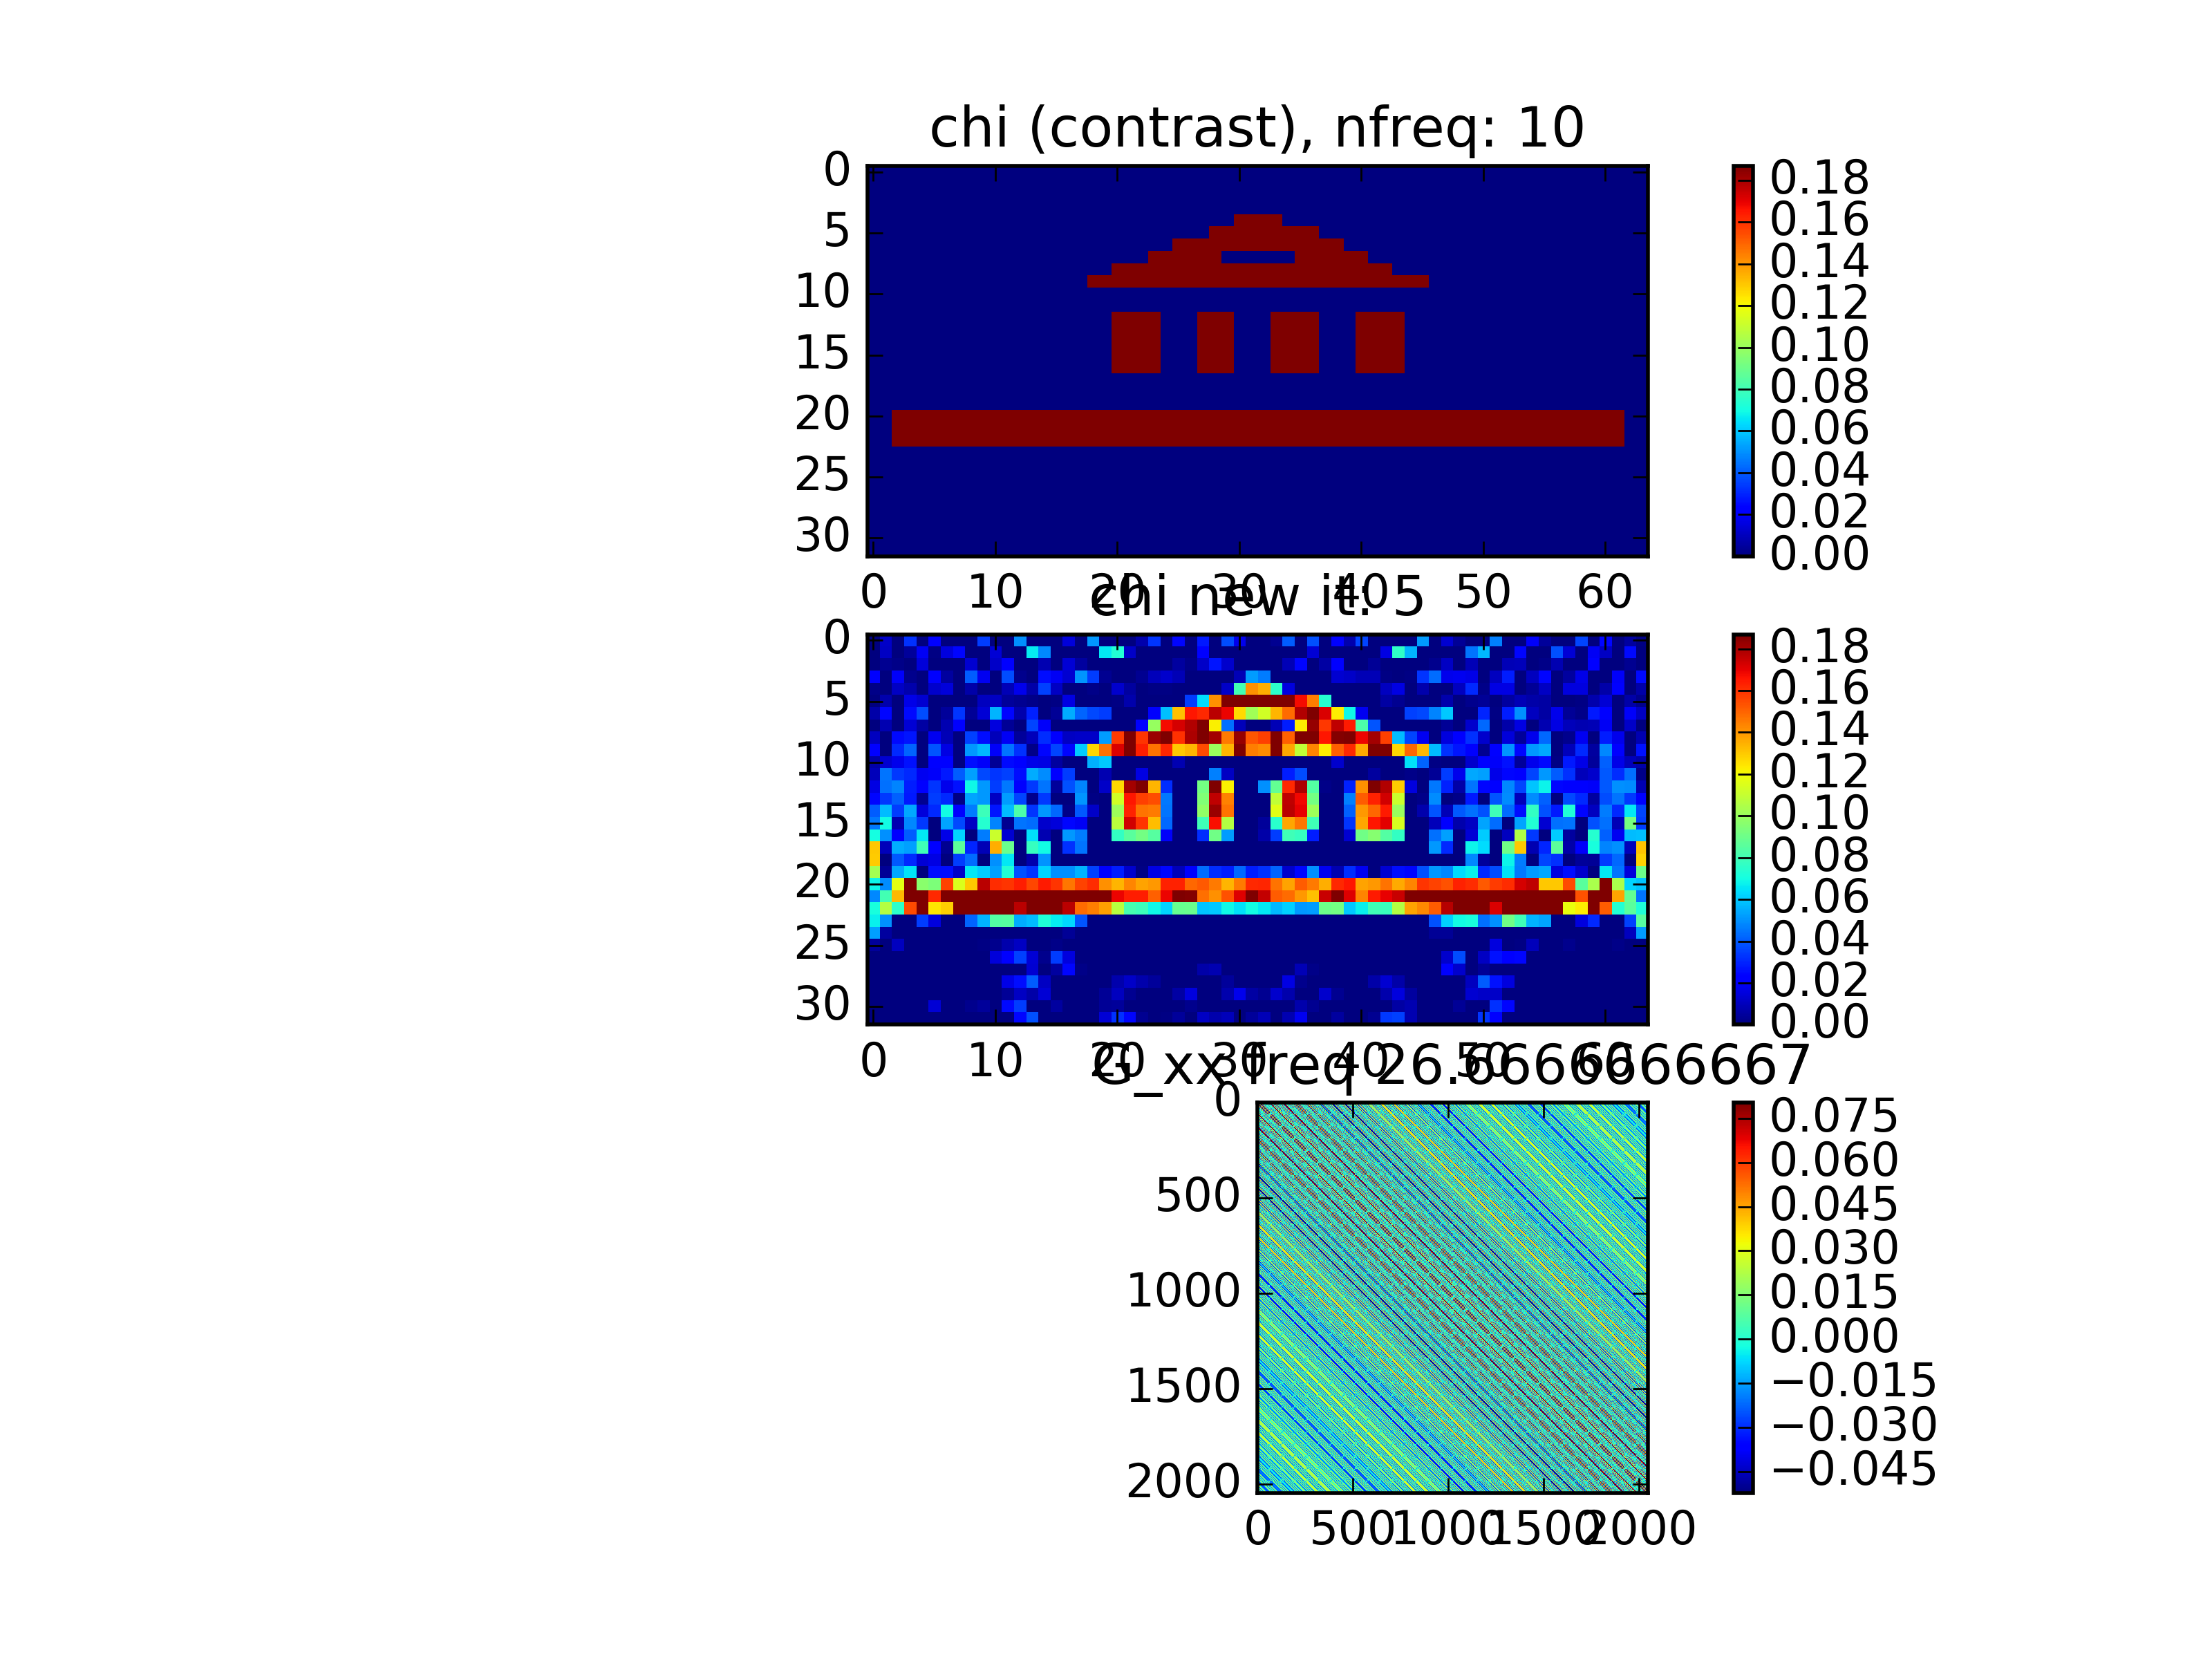
\includegraphics[scale=0.75]{Chi_est_it04.png}
  \caption{Chi estimation Result 5}
  \label{fig:fig8}
\end{figure}

\clearpage

\section{Appendices}
\subsection{Derivation of the functional derivative of the error functional}
\label{deriveerrorfunctional}
\begin{eqnarray*}
\partder{F(\mathbf{\chi}, \mathbf{d})}{\mathbf{\chi}} & = & \lim_{\epsilon \rightarrow 0} \frac{F(\mathbf{\chi} + \epsilon \mathbf{d}) - F(\mathbf{\chi})}{\epsilon} \\
& = & \lim_{\epsilon \rightarrow 0} \frac{\eta}{\epsilon} \int \left(p_{\text{data}} - \left[\mathcal{K}_\chi \right] - \epsilon \left[\mathcal{K}_\mathbf{d} \right] \right) \left(p_{\text{data}} - \left[\mathcal{K}_\chi \right] - \epsilon \left[\mathcal{K}_\mathbf{d} \right] \right)^{\dagger}\\
& \, \, \, \, \, \, \, \, \, \, \, \, \, \, \, \, \, \, \, \, \, \, \, \, \, \, \, - & \left(p_{\text{data}} - \left[\mathcal{K}_\chi \right] \right) \left(p_{\text{data}} - \left[\mathcal{K}_\chi \right] \right)^{\dagger} \df{\xs} \df{\xr} \df{\omega} \\
& = & -\lim_{\epsilon \rightarrow 0} \frac{\eta}{\epsilon} \int \epsilon \left[ \left[\mathcal{K}_\mathbf{d} \right] \left(p_{\text{data}} - \left[\mathcal{K}_\chi \right]  \right)^{\dagger} + \left[\mathcal{K}_\mathbf{d} \right]^{\dagger} \left(p_{\text{data}} - \left[\mathcal{K}_\chi \right] \right) \right] \\
& \, \, \, \, \, \, \, \, \, \, \, \, \, \, \, \, \, \, \, \, \, \, \, \, \, \, \, - & \epsilon^2 \left[\mathcal{K}_\mathbf{d} \right] \left[\mathcal{K}_\mathbf{d} \right]^{\dagger} \df{\xs} \df{\xr} \df{\omega} \\
& = & -2 \eta \int \real{\left[\mathcal{K}_\mathbf{d} \right] \left(p_{\text{data}} - \left[\mathcal{K}_\chi \right]  \right)^{\dagger}} \df{\xs} \df{\xr} \df{\omega} \\
& = & -2 \eta \int \real{\left[\mathcal{K}_\mathbf{d} \right](\xr, \xs, \omega)^{\dagger} r (\xr, \xs, \omega)} \df{\xs} \df{\xr} \df{\omega}
\end{eqnarray*}

\subsection{Prefactors of the Total Cost Equation}
\label{totalcostprefactors}
\begin{equation} \label{eq:eq24} \mathcal{A}_2 = \eta \int \int \int \mid \mathcal{K} \zeta_n \mid^2 d\vec{x_s}d\vec{x_r}d\omega \end{equation}

\begin{equation} \label{eq:eq25} \mathcal{A}_1 = -2 \eta \real{\int \int \int r^{\star}_{n-1} \mid \mathcal{K} \zeta_n \mid d\vec{x_s}d\vec{x_r}d\omega} , \hat{E} \end{equation}

\begin{equation} \label{eq:eq26} \mathcal{A}_0 = \eta \int \int \int \mid r_{n-1} \mid^2 d\vec{x_s}d\vec{x_r}d\omega =  \mathcal{F}^{data}_{n-1} , \hat{E} \end{equation}

\begin{equation} \label{eq:eq27} \mathcal{B}_2 = \mid \mid b_n \nabla \zeta_n \mid \mid^{2}_D , \hat{E} \end{equation}

\begin{equation} \label{eq:eq28} \mathcal{B}_1 = 2 < b_n \nabla\chi^{n-1}, b_n \nabla \zeta_n >_D, \hat{E} \end{equation}

\begin{equation} \label{eq:eq29} \mathcal{B}_0 = \mid \mid b_n \nabla \chi^{n-1} \mid \mid^{2}_D + \delta^{2}_{n-1} \mid \mid b_n \mid \mid^{2}_D \end{equation}

\end{document}